% ============================================================
%  TMSD — The Complete Self-Study Report
%  A4 article. Assumes no prior knowledge: every concept built
%  from the ground up, every equation translated to English.
%  Figures: upload the report/figures/ folder alongside this file.
%  Compile with pdfLaTeX on Overleaf.
% ============================================================
\documentclass[11pt,a4paper]{article}

\usepackage[margin=2.4cm]{geometry}
\usepackage{amsmath,amssymb,amsthm,bm}
\usepackage{cancel}
\usepackage{graphicx}
\graphicspath{{figures/}}
\usepackage{booktabs}
\usepackage{xcolor}
\usepackage{tikz}
\usetikzlibrary{arrows.meta,positioning,decorations.pathreplacing,calc}
\usepackage[most]{tcolorbox}
\usepackage{enumitem}
\usepackage[colorlinks=true, linkcolor=blue!60!black, urlcolor=blue!60!black]{hyperref}
\usepackage{microtype}

\definecolor{intu}{RGB}{42,120,214}
\definecolor{warn}{RGB}{205,72,54}
\definecolor{good}{RGB}{27,140,100}
\definecolor{golden}{RGB}{196,148,32}

% "Intuition" boxes: the plain-English translation of the math above them.
% Each accepts an optional key list, e.g. \begin{keyresult}[title=...]
\newtcolorbox{intuition}[1][]{colback=intu!6, colframe=intu!70, title=\textbf{Intuition},
  fonttitle=\small, left=2mm, right=2mm, top=1mm, bottom=1mm, boxrule=0.7pt, #1}
\newtcolorbox{keyresult}[1][]{colback=good!6, colframe=good!70, title=\textbf{Key result},
  fonttitle=\small, left=2mm, right=2mm, top=1mm, bottom=1mm, boxrule=0.7pt, #1}
\newtcolorbox{pitfall}[1][]{colback=warn!6, colframe=warn!70, title=\textbf{The flaw},
  fonttitle=\small, left=2mm, right=2mm, top=1mm, bottom=1mm, boxrule=0.7pt, #1}
\newtcolorbox{worked}[1][]{colback=black!4, colframe=black!45, title=\textbf{Worked example},
  fonttitle=\small, left=2mm, right=2mm, top=1mm, bottom=1mm, boxrule=0.7pt, #1}

\newtheorem{definition}{Definition}
\newtheorem{proposition}{Proposition}

\title{\textbf{Skills Nobody Taught}\\[2mm]
\Large Transport-Metric Skill Discovery on Granular Media:\\ the complete self-study report}
\author{Azfar Azdi Arfakhsyad}
\date{July 2026}

\begin{document}
\maketitle

\begin{abstract}
\noindent
This report documents, from first principles, a research campaign into
\emph{unsupervised skill discovery} --- teaching a robot to invent useful behaviors
with no rewards and no demonstrations --- applied for the first time to
\emph{granular material} (an excavator digging soil). It is written to be
self-contained: every mathematical tool (probability, entropy, mutual information,
reinforcement learning, optimal transport, constrained optimization) is built up
from zero before it is used. We cover the three landmark prior methods (DIAYN,
DADS, METRA) and their flaws; our proposed method (TMSD) and its two ingredients;
all nine experiments with their data; the falsification of our own original
hypothesis; the discovery that replaced it (a two-ingredient law and a
``slow-state'' failure taxonomy); and an honest account of what the method can and
cannot do. 33 training runs, $\approx$70 GPU-hours, one desktop GPU.
\end{abstract}

\medskip
\begin{center}
\begin{minipage}{0.86\linewidth}\small
\textbf{How to read this report.} Sections 2--3 build the mathematical toolkit
(skip them if you know information theory and RL; return whenever a symbol
bites). Section 4 is the intellectual history --- three methods, three flaws.
Section 5 builds optimal transport from a sand pile. Section 6 states our
method. Section 7 is the heart: nine experiments in chronological order,
including the death of our own hypothesis and what replaced it. Sections 8--9:
what is new, what is broken, what is next. Boxes: \textcolor{intu}{blue} =
plain-English intuition, \textcolor{black!60}{gray} = worked numeric example,
\textcolor{good}{green} = a result to remember, \textcolor{warn}{red} = a flaw
that matters later. Every figure is generated from the actual experiment data
(\texttt{report/make\_figures.py}).
\end{minipage}
\end{center}

\tableofcontents
\newpage

% ============================================================
\section{The problem in plain language}
% ============================================================

Robots today learn tasks the way a dog learns tricks: a human defines a
\emph{reward} --- a number that goes up when the robot does the right thing ---
and the robot fumbles around until it finds behavior that makes the number go up.
This works, but it has a painful catch: \textbf{someone has to write the reward},
and for every new task, a new reward. Writing rewards is genuinely hard. What is
the reward for ``knead this dough into a ball''? For ``grade this slope nicely''?
Engineers spend more time debugging reward functions than any other part of a
robot-learning system, because a robot will ruthlessly exploit any loophole in a
sloppy reward (this is called \emph{reward hacking}, and we will meet a
spectacular example of it later in this report --- an arm that ``dances'' for
enormous reward while doing zero useful work).

\medskip
\emph{Unsupervised skill discovery} (USD) asks a radical question: what if we give
the robot \textbf{no reward at all}? Instead we give it a knob --- a vector $z$
called the \emph{skill} --- and a single, task-free instruction:

\begin{center}
\emph{``Whatever you do, do something so different for each setting of the knob\\
that an observer could tell which setting you were given.''}
\end{center}

That's it. No definition of digging, walking, or grasping. The hope --- borne out
in practice --- is that in order to be \emph{distinguishably different}, the robot
must actually \emph{do} things: crawl left vs.\ crawl right, jump vs.\ crouch.
Behaviors emerge the way a child's sandbox repertoire emerges: not because anyone
defined ``dig,'' but because doing distinct things is the game itself. Afterwards,
the knob becomes a steering wheel: to make the robot do skill-$z$-like things, set
the knob to $z$.

\medskip
Prior to this project, USD had been demonstrated on robots moving \emph{their own
bodies} (locomotion) and rigid objects. It had never been shown on
\textbf{materials} --- soil, sand, dough --- which is precisely where reward
design is hardest and USD would be most valuable. Our testbed: a simulated
excavator arm over a bed of $\sim$1200 physically simulated soil grains. The
question: \emph{can it invent digging?}

% ============================================================
\section{Mathematical toolkit I: probability, surprise, and information}
% ============================================================

Everything in this field is built from a small set of probability ideas. We build
them here honestly, because the differences between the methods we study
\emph{are} differences between these quantities.

\subsection{Random variables, distributions, expectation}

A \emph{random variable} $X$ is a quantity whose value we are uncertain about ---
the roll of a die, the position of a soil grain. Its \emph{distribution} $p(x)$
assigns each possible value a probability (or, for continuous quantities, a
probability \emph{density}). Two facts we use constantly:
\[
\sum_x p(x) = 1
\qquad\text{and}\qquad
\mathbb{E}[f(X)] \;=\; \sum_x p(x)\, f(x),
\]
the \emph{expectation}: the average of $f$ over many samples of $X$, weighted by
how likely each value is. When you see $\mathbb{E}[\cdot]$ anywhere in this
report, read it as ``the average value of the thing inside, in the long run.''

\subsection{Entropy: measuring uncertainty}

\begin{definition}[Entropy]
$H(X) = -\sum_x p(x) \log p(x) = \mathbb{E}[-\log p(X)]$.
\end{definition}

The quantity $-\log p(x)$ is the \emph{surprise} of seeing $x$: rare events
(small $p$) are very surprising (large $-\log p$); certain events ($p=1$) carry
zero surprise. Entropy is therefore \textbf{average surprise} --- how unpredictable
$X$ is overall.

\begin{worked}
\textbf{The case, drawn.} Three coins; each bar is the probability of an
outcome. Wider spread of probability $=$ more uncertainty $=$ more entropy.

\begin{center}
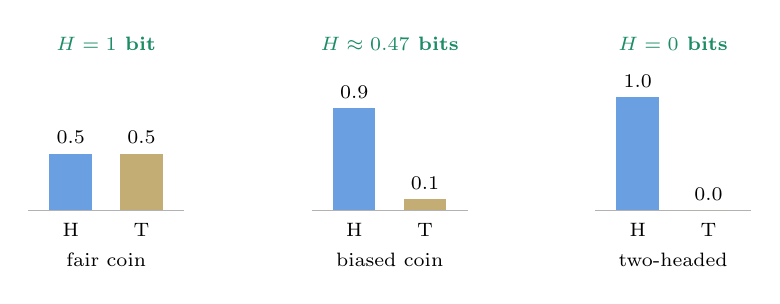
\begin{tikzpicture}[scale=0.9, every node/.style={font=\scriptsize}]
\foreach \x/\ph/\pt/\name/\hval in {0/0.5/0.5/fair coin/{$H=1$ bit},
                                    4/0.9/0.1/biased coin/{$H\approx0.47$ bits},
                                    8/1.0/0.0/two-headed/{$H=0$ bits}}{
  \draw[gray!60] (\x,0) -- (\x+2.2,0);
  \fill[intu!70]  (\x+0.3,0) rectangle (\x+0.9,\ph*1.6);
  \fill[golden!80!black!60] (\x+1.3,0) rectangle (\x+1.9,\pt*1.6);
  \node at (\x+0.6,-0.28) {H};
  \node at (\x+1.6,-0.28) {T};
  \node[above] at (\x+0.6,\ph*1.6) {\ph};
  \node[above] at (\x+1.6,\pt*1.6) {\pt};
  \node at (\x+1.1,-0.7) {\name};
  \node[good, font=\scriptsize\bfseries] at (\x+1.1,2.35) {\hval};
}
\end{tikzpicture}

{\scriptsize\emph{Legend: blue bar $=$ probability of heads; yellow bar $=$
probability of tails; green number $=$ the entropy we are about to compute.}}
\end{center}

\textbf{Solved step by step} (logs base 2, so the unit is bits):
\begin{enumerate}[leftmargin=6mm, itemsep=0mm]
\item \emph{Fair coin.} Surprise of H: $-\log_2 \tfrac12 = 1$. Surprise of T:
also $1$. Average with weights $\tfrac12,\tfrac12$:
$H = \tfrac12(1) + \tfrac12(1) = \mathbf{1\ bit}$.
\item \emph{Biased coin} ($p_\text{H}{=}0.9$). Surprise of H:
$-\log_2 0.9 \approx 0.152$ (common, barely surprising). Surprise of T:
$-\log_2 0.1 \approx 3.32$ (rare, very surprising). Weighted average:
$H = 0.9(0.152) + 0.1(3.32) \approx \mathbf{0.47\ bits}$ --- the rare outcome
is very surprising but rarely happens, so average surprise is \emph{low}.
\item \emph{Two-headed.} Only H can occur, surprise $-\log_2 1 = 0$:
$H = \mathbf{0\ bits}$. Certainty carries no information.
\end{enumerate}
Matching the picture: the flatter the bars, the higher the green number.
Entropy peaks when all outcomes are equally likely.
\end{worked}

\subsection{Conditional entropy and mutual information}

$H(X \mid Y)$ is the average surprise remaining about $X$ \emph{after you are
told} $Y$. If $Y$ tells you a lot about $X$, little surprise remains.

\begin{definition}[Mutual information]
\[
I(X;Y) \;=\; H(X) - H(X \mid Y).
\]
\end{definition}

\begin{intuition}
Mutual information is \textbf{how much your uncertainty about $X$ drops when you
learn $Y$} --- measured in bits. $I = 0$: independent. $I = H(X)$: $Y$ tells you
$X$ exactly. Crucially, MI only cares about \emph{distinguishability}, never about
\emph{magnitude}: if two skills differ by a soil grain displaced one millimeter,
but that millimeter is \emph{reliably} there, MI is just as satisfied as if they
had moved a whole dune. Keep this in mind --- it is the exact seed of DIAYN's
failure on soil.
\end{intuition}

\begin{worked}
\textbf{The case, drawn.} Two skills, $z \in \{A, B\}$, equally likely. Two
scenarios for what the skills actually \emph{do}:

\begin{center}
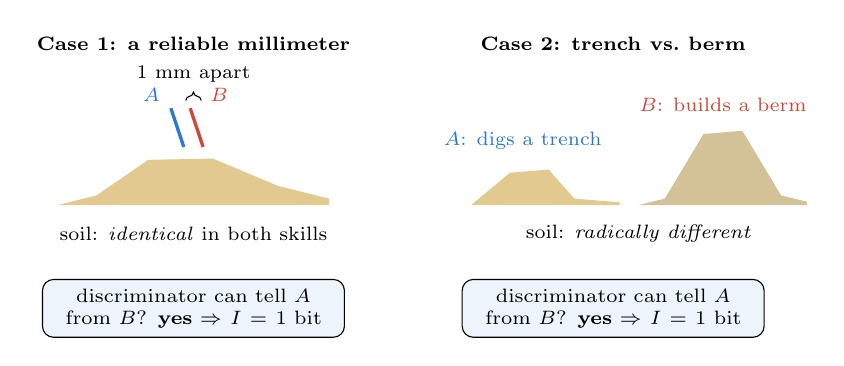
\begin{tikzpicture}[scale=0.82, every node/.style={font=\scriptsize}]
% ---- Case 1: 1 mm difference
\node[font=\scriptsize\bfseries] at (2.1,2.5) {Case 1: a reliable millimeter};
\fill[golden!50] (0,0) -- (0.6,0.15) -- (1.4,0.7) -- (2.4,0.72) -- (3.4,0.3) -- (4.2,0.1) -- (4.2,0) -- cycle;
\draw[very thick, intu] (1.75,1.5) -- (1.95,0.9);   % bucket A
\draw[very thick, warn] (2.05,1.5) -- (2.25,0.9);   % bucket B
\node[intu] at (1.45,1.7) {$A$};
\node[warn] at (2.5,1.7) {$B$};
\draw[decorate, decoration={brace, amplitude=3pt}] (1.98,1.62) -- (2.22,1.62)
  node[midway, above=3pt] {1 mm apart};
\node at (2.1,-0.45) {soil: \emph{identical} in both skills};
% ---- Case 2: trench vs berm
\node[font=\scriptsize\bfseries] at (8.6,2.5) {Case 2: trench vs.\ berm};
\fill[golden!50] (6.4,0) -- (7.0,0.5) -- (7.6,0.55) -- (8.0,0.1) -- (8.6,0.05)
  -- (8.7,0.05) -- (8.7,0) -- cycle;
\node[intu] at (7.2,1.0) {$A$: digs a trench};
\fill[golden!80!black!45] (9.0,0) -- (9.4,0.1) -- (10.0,1.1) -- (10.6,1.15)
  -- (11.2,0.15) -- (11.6,0.05) -- (11.6,0) -- cycle;
\node[warn] at (10.3,1.55) {$B$: builds a berm};
\node at (9.0,-0.45) {soil: \emph{radically different}};
% ---- verdict row
\node[draw, rounded corners, fill=intu!8, text width=3.6cm, align=center] at (2.1,-1.6)
  {discriminator can tell $A$ from $B$? \textbf{yes} $\Rightarrow I = 1$ bit};
\node[draw, rounded corners, fill=intu!8, text width=3.6cm, align=center] at (8.6,-1.6)
  {discriminator can tell $A$ from $B$? \textbf{yes} $\Rightarrow I = 1$ bit};
\end{tikzpicture}

{\scriptsize\emph{Legend: yellow $=$ soil; blue/red strokes $=$ where skill
$A$/$B$ leaves the bucket; the boxes give MI's verdict. MI scores both cases
identically.}}
\end{center}

\textbf{Solved step by step:}
\begin{enumerate}[leftmargin=6mm, itemsep=0mm]
\item Skills are equally likely, so before observing anything,
$H(Z) = -\tfrac12\log_2\tfrac12 - \tfrac12\log_2\tfrac12 = 1$ bit of
uncertainty about which skill is running.
\item \emph{Case 1.} The sensor resolves the millimeter, and the millimeter is
\emph{reliable} (always there). Seeing the state, you know the skill with
certainty: the remaining uncertainty is $H(Z \mid S) = 0$.
\item Therefore $I(S;Z) = H(Z) - H(Z\mid S) = 1 - 0 = \mathbf{1}$ \textbf{bit}
--- the \emph{maximum possible} for two skills.
\item \emph{Case 2.} A trench and a berm are also perfectly distinguishable:
again $H(Z \mid S) = 0$, again $I(S;Z) = \mathbf{1}$ \textbf{bit}.
\item Compare: $1 = 1$. \textbf{MI cannot prefer the trench over the
millimeter.} It measures \emph{distinguishability}, which saturates, not
\emph{magnitude of change}, which does not. Any method whose reward is MI
inherits this indifference --- and on soil we later measure exactly this
failure (Experiment 6).
\end{enumerate}
\end{worked}

% ============================================================
\section{Mathematical toolkit II: reinforcement learning in one section}
% ============================================================

\subsection{The loop}

At each time step $t$, the agent sees a \emph{state} $s_t$ (for us: arm joint
angles, joint speeds, a coarse soil height profile --- 35 numbers), picks an
\emph{action} $a_t$ (3 numbers: velocity commands for the three arm joints), and
the world's physics produces the next state $s_{t+1}$ plus a reward $r_t$.

\begin{center}
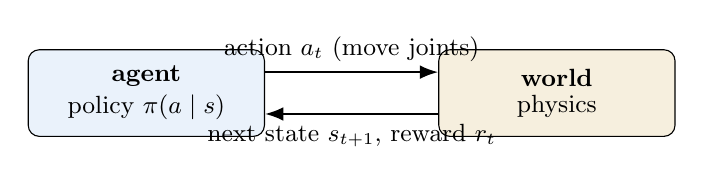
\begin{tikzpicture}[node distance=8mm and 22mm, every node/.style={font=\small}]
\node[draw, rounded corners, fill=intu!10, minimum width=3.0cm, minimum height=1.1cm] (agent)
  {\shortstack{\textbf{agent}\\ policy $\pi(a \mid s)$}};
\node[draw, rounded corners, fill=golden!15, minimum width=3.0cm, minimum height=1.1cm, right=of agent] (env)
  {\shortstack{\textbf{world}\\ physics}};
\draw[-Latex, thick] (agent.10) -- node[above]{action $a_t$ (move joints)} (env.170);
\draw[-Latex, thick] (env.190) -- node[below]{next state $s_{t+1}$, reward $r_t$} (agent.-10);
\end{tikzpicture}

{\scriptsize\emph{Legend: blue box $=$ the learner (a neural network mapping
state $\to$ action). Yellow box $=$ everything it cannot control (the
simulator). The loop repeats every 15\,ms of simulated time; learning means
adjusting the blue box so the stream of $r_t$ grows.}}
\end{center} The
agent's behavior rule is a \emph{policy} $\pi(a \mid s)$: a probability
distribution over actions given the state. The goal of RL:
\[
\max_\pi \; \mathbb{E}\Big[\, \textstyle\sum_{t=0}^{\infty} \gamma^t\, r_t \Big],
\qquad \gamma \in (0,1),
\]
maximize expected \emph{discounted return}. The discount $\gamma$ (we use $0.99$)
makes rewards now worth slightly more than rewards later, which keeps the sum
finite and encodes mild impatience.

\subsection{Value functions and the critic}

The \emph{Q-function} $Q^\pi(s,a)$ is the expected return if you take action $a$
in state $s$ and follow $\pi$ afterwards. It obeys a recursive consistency
condition (the Bellman equation):
\[
Q^\pi(s,a) \;=\; \mathbb{E}\big[\, r + \gamma\, Q^\pi(s', a') \,\big],
\quad a' \sim \pi(\cdot \mid s').
\]
Modern \emph{actor--critic} methods train two neural networks: a \emph{critic}
that estimates $Q$ by minimizing the mismatch between the two sides of this
equation, and an \emph{actor} (the policy) that adjusts itself to pick actions the
critic scores highly.

\subsection{SAC, the workhorse we use everywhere}

Soft Actor--Critic (SAC) is a standard, robust actor--critic algorithm with one
twist: it maximizes reward \emph{plus} the entropy of the policy,
\[
\max_\pi\; \mathbb{E}\Big[\textstyle\sum_t \gamma^t \big( r_t + \alpha\, H(\pi(\cdot \mid s_t)) \big)\Big].
\]
The entropy bonus keeps the policy exploratory (never prematurely certain), with
the temperature $\alpha$ auto-tuned. Implementation details we use: two critics
taking the minimum (avoids overestimation), a slowly-updated ``target'' copy of
the critics (stabilizes the bootstrap), and a replay buffer of past transitions
that gradient updates are sampled from. Every method compared in this report uses
\textbf{the exact same SAC machinery} --- the methods differ only in where $r_t$
comes from.

\subsection{Skill-conditioning}

In USD there is no external $r_t$. Instead: at the start of each episode a skill
$z$ is drawn at random from a fixed prior (ours: uniform on the unit sphere in
$\mathbb{R}^4$, i.e.\ a random direction), the policy becomes $\pi(a \mid s, z)$
--- the same network, with $z$ appended to its input --- and the reward is
\emph{manufactured} by the method itself to make behaviors depend on $z$. The next
section is the story of three ways to manufacture that reward, and what each one
gets wrong.

% ============================================================
\section{The three landmark methods, and the flaw in each}
% ============================================================

\subsection{DIAYN (2019): reward being identifiable}

\textbf{Objective.} Maximize the mutual information between states visited and
the skill: $I(S;Z) = H(Z) - H(Z \mid S)$. Since the skill prior is fixed, $H(Z)$
is constant, so the job is to \emph{minimize} $H(Z \mid S)$ --- make the skill
easy to guess from the state.

\textbf{Mechanism.} There is a snag: $H(Z \mid S)$ contains the \emph{posterior}
$p(z \mid s)$ --- ``given this state, which skill produced it?'' --- which nobody
knows. The fix is the \emph{variational bound}, a two-line derivation worth
seeing once. For \emph{any} approximating distribution $q_\varphi(z \mid s)$
(a neural network with parameters $\varphi$):
\[
\mathbb{E}\big[\log p(z \mid s)\big]
\;=\; \mathbb{E}\big[\log q_\varphi(z \mid s)\big]
\;+\; \underbrace{\mathbb{E}\big[\log \tfrac{p(z \mid s)}{q_\varphi(z \mid s)}\big]}_{\text{a KL divergence } \ge\, 0}
\;\;\ge\;\; \mathbb{E}\big[\log q_\varphi(z \mid s)\big].
\]
(The dropped term is a \emph{Kullback--Leibler divergence}, an average
log-ratio between two distributions; it is provably never negative, and is zero
exactly when $q_\varphi$ equals the true posterior.) So the unknowable quantity
is \emph{at least} the knowable one: train the discriminator $q_\varphi$ to
guess skills well, and you get an ever-tightening lower bound on the MI.
The per-step reward is then
\[
r_t \;=\; \log q_\varphi(z \mid s_{t+1}) \;-\; \log p(z),
\]
positive when the discriminator recognizes your skill better than chance.
\begin{intuition}
Two players cooperate. The \emph{policy} tries to visit states that scream
``I am skill $z$!''. The \emph{discriminator} learns to hear the scream. Reward is
high when the discriminator confidently guesses right. Behaviors must therefore
spread out over states --- each skill claims its own territory.
\end{intuition}

\begin{center}
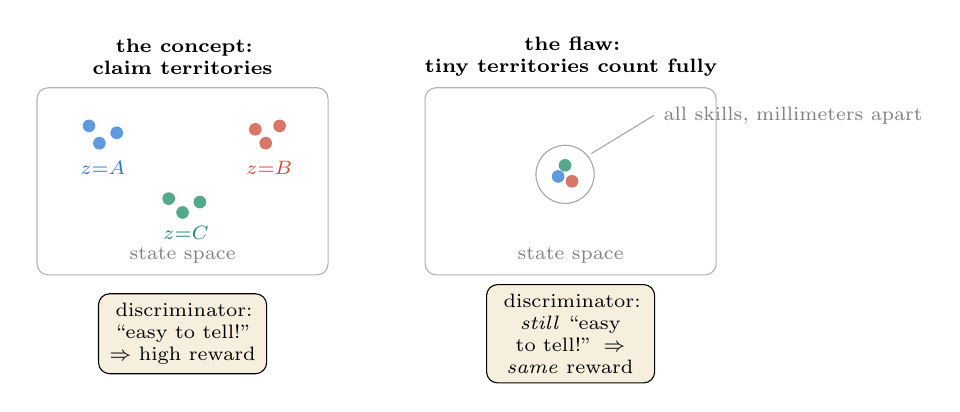
\begin{tikzpicture}[scale=0.88, every node/.style={font=\scriptsize}]
% ---- left: the concept
\node[font=\scriptsize\bfseries, text width=3.7cm, align=center] at (2.1,3.15)
  {the concept:\\ claim territories};
\draw[rounded corners, gray!60] (0,0) rectangle (4.2,2.7);
\node[gray] at (2.1,0.28) {state space};
\fill[intu!75]  (0.9,1.9) circle (2.6pt) (1.15,2.05) circle (2.6pt) (0.75,2.15) circle (2.6pt);
\fill[warn!75]  (3.3,1.9) circle (2.6pt) (3.5,2.15) circle (2.6pt) (3.15,2.1) circle (2.6pt);
\fill[good!75]  (2.1,0.9) circle (2.6pt) (2.35,1.05) circle (2.6pt) (1.9,1.1) circle (2.6pt);
\node[intu] at (0.95,1.55) {$z{=}A$};
\node[warn] at (3.35,1.55) {$z{=}B$};
\node[good] at (2.15,0.6) {$z{=}C$};
\node[draw, rounded corners, fill=golden!15, text width=1.9cm, align=center]
  at (2.1,-0.85) {discriminator: ``easy to tell!'' $\Rightarrow$ high reward};
% ---- right: the flaw
\node[font=\scriptsize\bfseries, text width=3.7cm, align=center] at (7.7,3.15)
  {the flaw:\\ tiny territories count fully};
\draw[rounded corners, gray!60] (5.6,0) rectangle (9.8,2.7);
\node[gray] at (7.7,0.28) {state space};
\fill[intu!75] (7.52,1.42) circle (2.6pt);
\fill[warn!75] (7.72,1.35) circle (2.6pt);
\fill[good!75] (7.62,1.58) circle (2.6pt);
\draw[gray!70] (7.62,1.45) circle (0.42);
\draw[gray!70] (8.0,1.75) -- (8.9,2.3) node[right, gray]{all skills, millimeters apart};
\node[draw, rounded corners, fill=golden!15, text width=1.9cm, align=center]
  at (7.7,-0.85) {discriminator: \emph{still} ``easy to tell!'' $\Rightarrow$ \emph{same} reward};
\end{tikzpicture}

{\scriptsize\emph{Legend: dots $=$ states visited by each skill (one color per
skill). Left: skills spread across the state space --- discriminator happy.
Right: skills differ by a reliable hair's width --- discriminator \emph{equally}
happy, reward \emph{equally} maximal. Nothing in the objective prefers left
over right.}}
\end{center}

\begin{worked}
\textbf{DIAYN's reward, computed --- and its ceiling.} Two skills, uniform
prior $p(z) = \tfrac12$; reward $r = \log_2 q_\varphi(z \mid s) - \log_2 p(z)$
(base 2, so bits).
\begin{enumerate}[leftmargin=6mm, itemsep=0mm]
\item \emph{Early training:} the discriminator is unsure, $q = 0.6$.
$r = \log_2 0.6 - \log_2 0.5 = -0.74 - (-1) = \mathbf{+0.26}$ bits. Small
positive reward: keep separating.
\item \emph{Later:} skills are quite distinguishable, $q = 0.95$.
$r = \log_2 0.95 + 1 = \mathbf{+0.93}$ bits.
\item \emph{The ceiling:} even a perfect discriminator gives
$r = \log_2 1 + 1 = \mathbf{1}$ bit --- and no more, ever. The reward can
never exceed $\log_2 \tfrac{1}{p(z)}$.
\item \emph{The flaw, numerically:} the millimeter-skill from the previous
worked example already achieves $q \approx 1$, i.e.\ reward
$\approx$ the ceiling. Digging a trench instead would raise the reward by
$\approx \mathbf{0.00}$ bits. \textbf{Gradient toward more change: zero.}
That is saturation --- and on soil we measured the discriminator at $0.98$
cosine within the first few thousand steps, reward flat ever after
(Figure~\ref{fig:mechanisms}, middle).
\end{enumerate}
\end{worked}

\begin{pitfall}
Identifiable $\neq$ substantial. A skill that tilts one joint by one degree
\emph{and holds it} is perfectly identifiable. MI rewards
\textbf{distinguishability, not magnitude, and not continued change}: once states
are separable, the game is won and nothing pushes further. On our soil domain we
measured exactly this: the discriminator reached $0.98$ accuracy while soil
movement stayed at the ambient noise floor (Section~\ref{sec:mi2x2}). We call
this failure mode \textbf{saturation}.
\end{pitfall}

\subsection{DADS (2020): reward being predictable}

\textbf{Objective.} Skills should have \emph{modelable consequences}. Learn a
skill-conditioned dynamics model $q_\theta(s' \mid s, z)$ (``if I am doing skill
$z$ in state $s$, where do I land?''), and reward transitions that this model
predicts well \emph{under your own skill} but that look unlike other skills'
transitions:
\[
r_t \;=\; \log q_\theta(s_{t+1} \mid s_t, z)
\;-\; \log \frac{1}{L}\sum_{l=1}^{L} q_\theta(s_{t+1} \mid s_t, z_l),
\qquad z_l \sim p(z).
\]
The second term is the average prediction quality under $L$ \emph{randomly
drawn alternative skills}: your transition should be \emph{yours} --- predictable
given $z$, surprising given anything else.

\begin{intuition}
DIAYN asks ``can an observer tell skills apart by \emph{where you are}?''
DADS asks ``can an observer tell skills apart by \emph{how you move}?'' ---
and additionally demands that each skill's motion be regular enough to forecast,
which is what later makes planning with skills possible.
\end{intuition}

\begin{center}
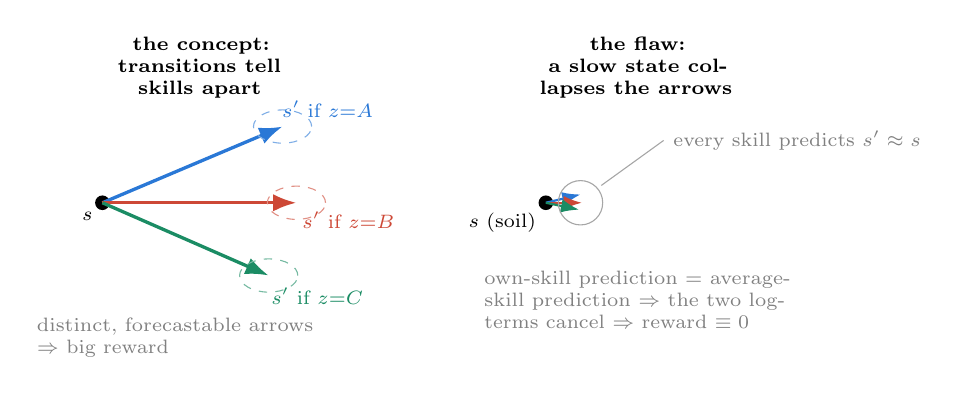
\begin{tikzpicture}[scale=0.88, every node/.style={font=\scriptsize}]
% ---- left: concept on a fast state
\node[font=\scriptsize\bfseries, text width=3.6cm, align=center] at (2.0,3.15)
  {the concept:\\ transitions tell skills apart};
\fill[black] (0.6,1.2) circle (3pt) node[below left]{$s$};
\draw[-Latex, very thick, intu] (0.6,1.2) -- (3.2,2.3);
\draw[intu!60, dashed] (3.2,2.3) ellipse (0.42 and 0.24);
\node[intu] at (3.85,2.55) {$s'$ if $z{=}A$};
\draw[-Latex, very thick, warn] (0.6,1.2) -- (3.4,1.2);
\draw[warn!60, dashed] (3.4,1.2) ellipse (0.42 and 0.24);
\node[warn] at (4.15,0.95) {$s'$ if $z{=}B$};
\draw[-Latex, very thick, good] (0.6,1.2) -- (3.0,0.15);
\draw[good!60, dashed] (3.0,0.15) ellipse (0.42 and 0.24);
\node[good] at (3.7,-0.15) {$s'$ if $z{=}C$};
\node[gray, text width=3.6cm] at (1.7,-0.75)
  {distinct, forecastable arrows $\Rightarrow$ big reward};
% ---- right: flaw on a slow state
\node[font=\scriptsize\bfseries, text width=3.9cm, align=center] at (8.3,3.15)
  {the flaw:\\ a slow state collapses the arrows};
\fill[black] (7.0,1.2) circle (3pt) node[below left]{$s$ (soil)};
\draw[-Latex, thick, intu] (7.0,1.2) -- (7.5,1.32);
\draw[-Latex, thick, warn] (7.0,1.2) -- (7.52,1.2);
\draw[-Latex, thick, good] (7.0,1.2) -- (7.48,1.1);
\draw[gray!70] (7.5,1.2) circle (0.32);
\draw[gray!70] (7.8,1.45) -- (8.7,2.1) node[right, gray]{every skill predicts $s' \approx s$};
\node[gray, text width=4.2cm] at (8.5,-0.2)
  {own-skill prediction $=$ average-skill prediction $\Rightarrow$ the two
   log-terms cancel $\Rightarrow$ reward $\equiv 0$};
\end{tikzpicture}

{\scriptsize\emph{Legend: black dot $=$ current state; colored arrows $=$ each
skill's predicted next state (dashed ellipse $=$ prediction spread). Left,
locomotion: skills produce different, forecastable futures. Right, soil: the
material barely moves per step, so all three arrows land on the same spot ---
there is nothing to be ``more predictable than the others'' about.}}
\end{center}

\begin{worked}
\textbf{DADS's reward, computed twice.} Log-densities of a Gaussian prediction
model: $\log q \propto -\text{error}^2 / (2\sigma^2)$; take $\sigma = 1$ and
$L$ alternative skills. Reward $r = \log q(s' \mid s, z) - \log
\frac{1}{L}\sum_l q(s' \mid s, z_l)$.
\begin{enumerate}[leftmargin=6mm, itemsep=0mm]
\item \emph{Fast state (locomotion-like).} Your own skill predicts the
transition well: error $0.1 \Rightarrow \log q_z = -0.005$. Other skills
predict it badly: error $1.0 \Rightarrow \log q_{z_l} = -0.5$ each. Reward
$r = -0.005 - (-0.5) = \mathbf{+0.495}$. Positive: your motion is
\emph{yours}. Learning proceeds.
\item \emph{Slow state (soil).} The soil barely changes: $s' - s \approx 0$.
Every skill's model predicts ``no change'' perfectly: own error $\approx 0$
\emph{and} alternatives' error $\approx 0$. Reward
$r = 0 - 0 = \mathbf{0.000}$. Not small --- \emph{exactly} zero, because the
two terms are the same number.
\item There is no gradient in step 2 and never will be: to escape, the policy
would need to \emph{already} be moving soil in skill-distinct ways --- which
is precisely what the zero reward fails to teach. Chicken and egg; the
measured result is a flatline at $0.000$ for 200{,}000 steps
(Figure~\ref{fig:mechanisms}, bottom).
\end{enumerate}
\end{worked}

\begin{pitfall}
The signal lives entirely in the \textbf{per-step change} $s' - s$. Materials
are \emph{slow}: most steps, the soil barely changes. Then $s' \approx s$ is
trivially predictable \emph{under every skill}, the two log-terms cancel, and the
reward is identically zero --- not small, \emph{zero}. We measured DADS-with-soil
rewards at $0.000$ for an entire 200{,}000-step run
(Figure~\ref{fig:mechanisms}, bottom panel). We call this failure mode
\textbf{starvation}.
\end{pitfall}

\subsection{METRA (2024): reward going far}

\textbf{Objective.} Learn a map $\phi \colon \text{states} \to \mathbb{R}^D$
(the \emph{representation}) and make each skill travel along its own direction in
that latent space:
\begin{equation}
\max_{\pi, \phi} \;\; \mathbb{E}\big[ (\phi(s_{t+1}) - \phi(s_t))^{\!\top} z \big]
\qquad \text{subject to} \qquad
\|\phi(s) - \phi(s')\| \;\le\; d(s, s') ,
\label{eq:metra}
\end{equation}
where $z$ is a unit vector and $d$ is some notion of distance between states.

\textbf{Why the constraint must exist.} Without it there is a fatal cheat:
$\phi$ could simply \emph{stretch} --- multiply itself by 1000 --- and every
reward would grow 1000-fold with no behavioral change. The constraint pins the
latent space to reality: \emph{one unit of latent motion must be backed by at
least one unit of real motion}, as measured by $d$. METRA's choice of $d$ is the
\emph{temporal} distance (roughly: adjacent steps are at distance $\le 1$).

\textbf{How a constraint is enforced in practice (Lagrangian duality, gently).}
You cannot tell a neural network ``obey this inequality.'' Instead you convert
the constrained problem into an unconstrained one with a \emph{price}. Define
the penalized objective
\[
\mathcal{L}(\phi, \lambda) \;=\;
\underbrace{\mathbb{E}\big[(\phi(s')-\phi(s))^\top z\big]}_{\text{reward}}
\;+\; \lambda \cdot
\underbrace{\mathbb{E}\big[\min\big(\epsilon,\; d^2 - \|\phi(s)-\phi(s')\|^2\big)\big]}_{\text{constraint slack (positive = obeyed)}} .
\]
$\lambda \ge 0$ is a learnable \emph{price of violation}: while the constraint is
violated (slack negative) the price rises, punishing $\phi$ harder; when obeyed,
the price falls. The system self-tunes to run right at the boundary --- which is
exactly where you want it, since reward grows with latent distance and latent
distance is capped by real distance. (We watch $\lambda$ throughout training as
a health signal; ours stabilizes around $\lambda \approx 30$.)

\begin{intuition}
Think of $\lambda$ as a \emph{fine} set by a regulator. The network wants to
stretch its map (more stretch $=$ more reward); stretching past what physical
distance justifies incurs the fine. If networks keep cheating, the regulator
raises the fine until they stop; if nobody cheats, the fine decays so it doesn't
distort honest behavior. At equilibrium the map is stretched \emph{exactly} to
the legal limit --- taut like a drumhead --- which is what makes latent distances
meaningful measurements of real distances.
\end{intuition}

\textbf{The telescoping property --- the single most load-bearing equation in
this report.} Sum the per-step rewards over an episode:
\begin{equation}
\sum_{t=0}^{T-1} (\phi(s_{t+1}) - \phi(s_t))^{\!\top} z
\;=\; \big(\phi(s_T) - \phi(s_0)\big)^{\!\top} z .
\label{eq:telescope}
\end{equation}
To see it, write out three steps and watch the middle terms annihilate:
\[
(\phi_1 - \phi_0)^\top z + (\phi_2 - \phi_1)^\top z + (\phi_3 - \phi_2)^\top z
= (\cancel{\phi_1} - \phi_0 + \cancel{\phi_2} - \cancel{\phi_1} + \phi_3 - \cancel{\phi_2})^\top z
= (\phi_3 - \phi_0)^\top z .
\]
Every intermediate position appears once with $+$ and once with $-$ (a
collapsing telescope). The total reward of an episode depends \emph{only on
where you ended relative to where you started}: wiggling back and forth earns
nothing net; a step backward \emph{costs} exactly what the forward step earned.

\begin{center}
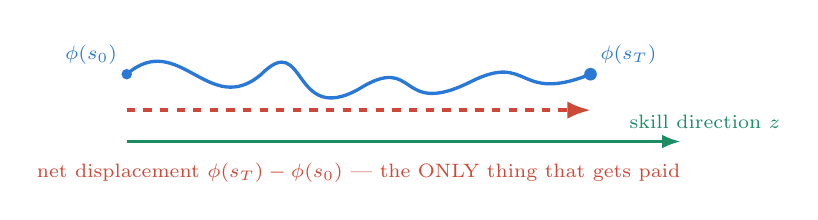
\begin{tikzpicture}[scale=0.95, every node/.style={font=\scriptsize}]
% skill direction
\draw[-Latex, thick, good] (0,0) -- (7.4,0)
  node[above left=1pt and -14mm]{skill direction $z$};
% wiggly latent path
\draw[intu, very thick]
  (0,0.9) .. controls (0.7,1.5) and (1.1,0.3) .. (1.8,0.9)
          .. controls (2.4,1.5) and (2.2,0.2) .. (3.1,0.7)
          .. controls (3.9,1.2) and (3.6,0.3) .. (4.6,0.8)
          .. controls (5.4,1.2) and (5.2,0.5) .. (6.2,0.9);
\fill[intu] (0,0.9) circle (2pt) node[above left]{$\phi(s_0)$};
\fill[intu] (6.2,0.9) circle (2.4pt) node[above right]{$\phi(s_T)$};
% net displacement arrow
\draw[-Latex, very thick, warn, dashed] (0,0.42) -- (6.2,0.42);
\node[warn, font=\scriptsize] at (3.1,-0.42)
  {net displacement $\phi(s_T)-\phi(s_0)$ --- the ONLY thing that gets paid};
\end{tikzpicture}

{\scriptsize\emph{Legend: blue curve $=$ the wandering latent trajectory over
one episode (all its wiggles cancel in the reward sum). Red dashed arrow $=$
the net start-to-end displacement; the episode's total reward is this arrow's
length along the green skill direction $z$.}}
\end{center}

This is why we will call distance-maximizing objectives \emph{cumulative} ---
and it is the property that will single-handedly decide the frontier comparison
in Section~7.

\begin{intuition}
DIAYN pays you for \emph{being recognizable}. DADS pays you for \emph{moving
recognizably}. METRA pays you for \textbf{net displacement} --- and, through the
constraint, latent displacement is backed by real-world distance. You cannot
micro-cheat; you must actually go somewhere and stay there.
\end{intuition}

\begin{center}
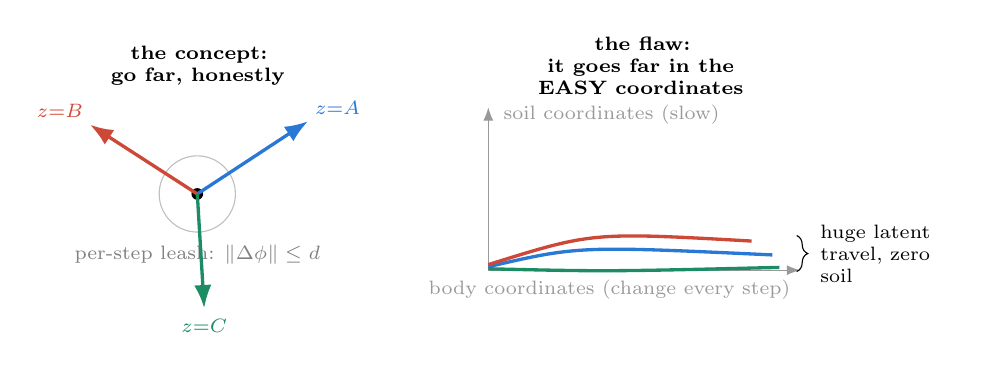
\begin{tikzpicture}[scale=0.88, every node/.style={font=\scriptsize}]
% ---- left: concept
\node[font=\scriptsize\bfseries, text width=3.4cm, align=center] at (1.9,3.15)
  {the concept:\\ go far, honestly};
\draw[gray!50] (1.9,1.3) circle (0.55);
\node[gray, below=1pt] at (1.9,0.75) {per-step leash: $\|\Delta\phi\| \le d$};
\fill[black] (1.9,1.3) circle (2.4pt);
\draw[-Latex, very thick, intu] (1.9,1.3) -- (3.5,2.35) node[above right=-2pt]{$z{=}A$};
\draw[-Latex, very thick, warn] (1.9,1.3) -- (0.35,2.3) node[above left=-2pt]{$z{=}B$};
\draw[-Latex, very thick, good] (1.9,1.3) -- (2.0,-0.35) node[below]{$z{=}C$};
% ---- right: flaw
\node[font=\scriptsize\bfseries, text width=4.4cm, align=center] at (8.3,3.15)
  {the flaw:\\ it goes far in the EASY coordinates};
\draw[-Latex, gray!80] (6.1,0.2) -- (10.6,0.2) node[below left]{body coordinates (change every step)};
\draw[-Latex, gray!80] (6.1,0.2) -- (6.1,2.55);
\node[gray!80, right] at (6.18,2.45) {soil coordinates (slow)};
\draw[very thick, intu]  (6.1,0.25) .. controls (7.4,0.55) .. (10.2,0.42);
\draw[very thick, warn]  (6.1,0.28) .. controls (7.6,0.75) .. (9.9,0.62);
\draw[very thick, good]  (6.1,0.22) .. controls (7.8,0.18) .. (10.3,0.24);
\draw[decorate, decoration={brace, amplitude=4pt}] (10.55,0.7) -- (10.55,0.18)
  node[midway, right=5pt, text width=1.6cm]{huge latent travel, zero soil};
\end{tikzpicture}

{\scriptsize\emph{Legend. Left: from the current latent position (black dot),
each skill pushes in its own direction; the gray circle is the per-step
constraint --- one unit of latent motion must be backed by real motion. Right:
when $\phi$ sees the full state, the cheap way to ``go far'' is along the body
axes, which move at every step; all skills race horizontally while the soil
axis stays untouched.}}
\end{center}

\begin{worked}
\textbf{METRA's reward, computed --- honest version and exploited version.}
Take skill $z = +1$ in a 1-D latent for arithmetic's sake.
\begin{enumerate}[leftmargin=6mm, itemsep=0mm]
\item \emph{Telescoping, with numbers.} Suppose over four steps
$\phi = 0 \to 0.3 \to 0.2 \to 0.6$. Per-step rewards:
$+0.3,\ -0.1,\ +0.4$. Sum $= \mathbf{0.6} = \phi_{\text{end}} -
\phi_{\text{start}}$. The backward wiggle ($-0.1$) was \emph{charged}, not
ignored: only net progress pays.
\item \emph{Our constraint ($d = W_2$ on soil).} Step moves $0.35$\,m of soil
transport $\Rightarrow$ $|\Delta\phi| \le 0.35$: latent progress is capped by
\emph{physical work}. Arm-waves move $0.000$\,m of soil $\Rightarrow$
$|\Delta\phi| \le 0$ $\Rightarrow$ reward for arm-waving
$= \mathbf{0}$, \emph{by construction}.
\item \emph{Vanilla METRA's constraint (temporal, $d \equiv 1$ per step).}
Any adjacent states are ``distance 1'' apart --- \emph{including} two states
that differ only in arm pose. So an arm-wave may earn up to $1$ latent unit
\emph{per step}: over a 200-step episode, up to $\mathbf{200}$ units of
latent travel with zero soil moved. Measured: its latent fan spans
$\pm 150$ (Figure~\ref{fig:latentcmp}) over untouched terrain --- within
$25\%$ of this back-of-envelope ceiling.
\end{enumerate}
\end{worked}

\begin{pitfall}
Go far --- \emph{in which part of the state?} The state contains the robot's own
body, and the body is the easiest thing in the world to move far. Every one of
these objectives, fed the full state, feasts on proprioception. In a
manipulation scene the result is an agent that develops elaborate arm
choreography and never touches the object --- documented by the CSD authors
(2023) as ``completely ignoring the object,'' and reproduced by us, quantified,
on soil (Section~\ref{sec:factorization}).
\end{pitfall}

% ============================================================
\section{Mathematical toolkit III: optimal transport}
% ============================================================
\label{sec:ot}

Our original idea needs one more mathematical instrument --- a beautiful one.
But first, a decoder for the three ``distances'' this report keeps comparing.

\subsection{Three rulers for the same question}

Everywhere in skill discovery, some quantity $d(s, s')$ must answer: \emph{how
different are two states?} The three candidate rulers give radically different
answers to the same pair of soil states --- and each has a blind spot the
experiments will exploit.

\paragraph{Euclidean distance: compare the lists, entry by entry.}
A soil state is a list of numbers (mass per column). Euclidean distance
subtracts the lists entry-wise, squares, sums, roots:
$d_{\text{euc}} = \sqrt{\sum_i (\mu_i - \nu_i)^2}$. It asks: \emph{``how much
does each column differ?''} --- and nothing else. \textbf{Blind spot:
geometry.} Take a pile occupying one column, and shift it. Shift by one column
or by fifty: in both cases the old column lost everything and some new column
gained everything, so \emph{the entry-wise difference is identical}. With
$\mu = (1,0,0,\ldots)$: shifting to column 2 gives
$d_{\text{euc}} = \sqrt{1^2 + 1^2} = 1.41$; shifting to column 50 gives
\emph{the same} $1.41$. Near rearrangement and massive rearrangement ---
indistinguishable.

\paragraph{Temporal distance: count the steps.}
METRA's ruler. The distance between two states is (roughly) \emph{the number of
environment steps needed to get from one to the other}; in practice, states one
step apart are at distance $\le 1$. It asks: \emph{``how long does it take?''}
\textbf{Blind spot: content.} One time-step in which the bucket drags 100\,kg
of soil, and one time-step in which the arm twitches in the air, are the
\emph{same} distance: 1. The ruler prices effort in seconds, not in
consequences --- which is exactly the loophole the arm-dancing exploit drives
through (one latent unit per step, 200 steps, zero soil).

\paragraph{Wasserstein distance: price the earth-moving.}
The physical ruler, developed in the rest of this section. It asks:
\emph{``how much work --- mass $\times$ distance --- would a perfect bulldozer
need to turn one pile into the other?''} Shift a pile one column: cheap. Shift
it fifty columns: fifty times the work. Wave the arm: the pile is unchanged,
distance zero. Its answers are denominated in physical units.
\textbf{Blind spot} (found by our experiments, Section 7): it prices soil work
correctly, but as a \emph{learning signal} it can be too faint to bootstrap
from --- correctness and trainability are different virtues.

\begin{center}
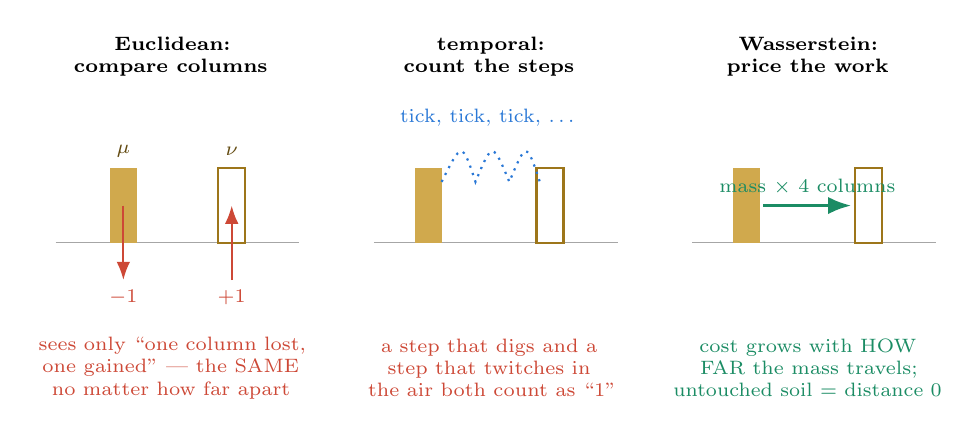
\begin{tikzpicture}[scale=0.86, every node/.style={font=\scriptsize}]
% common: pile at col 2, shifted pile at col 6
% ---- panel 1: Euclidean
\node[font=\scriptsize\bfseries, text width=3.4cm, align=center] at (1.7,2.75)
  {Euclidean:\\ compare columns};
\draw[gray!70] (0,0) -- (3.6,0);
\fill[golden!80] (0.8,0) rectangle (1.2,1.1);
\draw[golden!80!black, thick] (2.4,0) rectangle (2.8,1.1);
\node[golden!50!black] at (1.0,1.35) {$\mu$};
\node[golden!50!black] at (2.6,1.35) {$\nu$};
\draw[-Latex, warn, thick] (1.0,0.55) -- (1.0,-0.55) node[below]{$-1$};
\draw[-Latex, warn, thick] (2.6,-0.55) node[below]{$+1$} -- (2.6,0.55);
\node[warn, text width=3.4cm, align=center] at (1.7,-1.85)
  {sees only ``one column lost, one gained'' --- the SAME no matter how far apart};
% ---- panel 2: temporal
\node[font=\scriptsize\bfseries, text width=3.4cm, align=center] at (6.4,2.75)
  {temporal:\\ count the steps};
\draw[gray!70] (4.7,0) -- (8.3,0);
\fill[golden!80] (5.3,0) rectangle (5.7,1.1);
\draw[golden!80!black, thick] (7.1,0) rectangle (7.5,1.1);
\draw[intu, thick, dotted] (5.7,0.9) .. controls (6.0,1.5) .. (6.2,0.9)
  .. controls (6.45,1.5) .. (6.7,0.9) .. controls (6.95,1.5) .. (7.15,0.9);
\node[intu] at (6.4,1.85) {tick, tick, tick, \dots};
\node[warn, text width=3.4cm, align=center] at (6.4,-1.85)
  {a step that digs and a step that twitches in the air both count as ``1''};
% ---- panel 3: Wasserstein
\node[font=\scriptsize\bfseries, text width=3.4cm, align=center] at (11.1,2.75)
  {Wasserstein:\\ price the work};
\draw[gray!70] (9.4,0) -- (13.0,0);
\fill[golden!80] (10.0,0) rectangle (10.4,1.1);
\draw[golden!80!black, thick] (11.8,0) rectangle (12.2,1.1);
\draw[-Latex, good, very thick] (10.45,0.55) -- (11.75,0.55)
  node[midway, above]{mass $\times$ 4 columns};
\node[good, text width=3.4cm, align=center] at (11.1,-1.85)
  {cost grows with HOW FAR the mass travels; untouched soil $=$ distance 0};
\end{tikzpicture}

{\scriptsize\emph{Legend: in every panel, the filled block is the pile now
($\mu$), the hollow block is the target pile ($\nu$), four columns to the
right. Three rulers, three verdicts on the same pair: Euclidean sees
``two columns changed'' (blind to the four-column gap); temporal sees
``however many ticks the machine needs'' (blind to what each tick did);
Wasserstein sees ``this much mass moved this far'' --- the physical answer.}}
\end{center}

\begin{intuition}
Same question, three currencies. Euclidean pays in \emph{pixels changed},
temporal pays in \emph{seconds spent}, Wasserstein pays in
\emph{tons-moved-times-meters}. Our original hypothesis was that the third
currency --- the only physical one --- would make skills better. The
experiments' surprise: within the working recipe, all three currencies buy the
same skills (Experiment 2), because the learned map ends up physically
calibrated \emph{no matter which currency trained it}. The currency that
matters is the one the \emph{conditioning} chooses: what $\phi$ is allowed to
see.
\end{intuition}

\subsection{The earth mover's problem}

You have a pile of sand shaped like $\mu$ and want a pile shaped like $\nu$
(same total mass). Moving one kilogram of sand a distance of one meter costs one
unit of work. \textbf{What is the cheapest total work?} That minimal cost is a
\emph{distance between the two shapes}: small if $\nu$ is a slight rearrangement
of $\mu$, large if mass must travel far. This is the \emph{Wasserstein distance},
also called the \emph{earth mover's distance} --- and for us the name is literal:
\textbf{our robot is the earth mover}, and its job description is this exact
integral.

\subsection{The formal definition}

\begin{definition}[Kantorovich formulation of $W_2$]
For distributions $\mu, \nu$ on $\mathbb{R}^n$:
\[
W_2(\mu,\nu) \;=\; \left( \min_{\gamma \in \Pi(\mu,\nu)}
\int \|x - y\|^2 \; d\gamma(x,y) \right)^{1/2},
\]
where $\Pi(\mu,\nu)$ is the set of \emph{transport plans}: joint distributions
$\gamma(x,y)$ whose marginals are $\mu$ and $\nu$. Read $\gamma(x,y)$ as ``how
much mass I ship from location $x$ to location $y$''; the marginal conditions say
you ship away exactly the pile you have and deliver exactly the pile you want.
\end{definition}

Why squared distance ($W_2$ rather than $W_1$)? Squared costs favor many short
moves over one long move, give the distance Riemannian-geometry structure
(geodesics, barycenters), and connect to fluid dynamics (Benamou--Brenier: $W_2$
is the minimum kinetic energy of a flow morphing $\mu$ into $\nu$). For this
report it suffices that $W_2$ is the standard choice with the richest theory.

Contrast with the \emph{Euclidean} distance between the piles' height profiles,
$\|\mu - \nu\|_2$: that compares the piles \textbf{column by column}, and is
blind to geometry --- a pile shifted 10\,cm and the same pile shifted 5\,m look
equally ``different,'' because in both cases each column changed. Wasserstein
knows the second rearrangement is fifty times more work.

\begin{worked}
\textbf{The case, drawn.} Sand as blocks on a number line; arrows are transport
plans (``ship this block there'').

\begin{center}
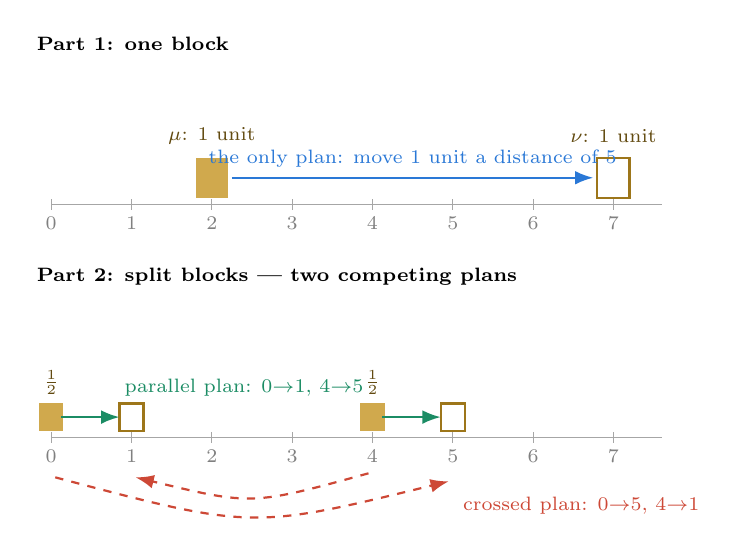
\begin{tikzpicture}[scale=1.02, every node/.style={font=\scriptsize}]
% ---- Part 1: single blocks
\node[font=\scriptsize\bfseries, anchor=west] at (-0.3,2.0) {Part 1: one block};
\draw[gray!70] (0,0) -- (7.6,0);
\foreach \x in {0,1,...,7} {\draw[gray!70] (\x,-0.07) -- (\x,0.07) node[below=3pt, gray]{\x};}
\fill[golden!80] (1.8,0.08) rectangle (2.2,0.58);
\node[golden!50!black] at (2,0.85) {$\mu$: 1 unit};
\draw[fill=white, draw=golden!80!black, thick] (6.8,0.08) rectangle (7.2,0.58);
\node[golden!50!black] at (7,0.85) {$\nu$: 1 unit};
\draw[-Latex, thick, intu] (2.25,0.33) -- (6.75,0.33)
  node[midway, above]{the only plan: move 1 unit a distance of 5};
% ---- Part 2: split blocks
\begin{scope}[yshift=-2.9cm]
\node[font=\scriptsize\bfseries, anchor=west] at (-0.3,2.0) {Part 2: split blocks --- two competing plans};
\draw[gray!70] (0,0) -- (7.6,0);
\foreach \x in {0,1,...,7} {\draw[gray!70] (\x,-0.07) -- (\x,0.07) node[below=3pt, gray]{\x};}
\fill[golden!80] (-0.15,0.08) rectangle (0.15,0.42);
\fill[golden!80] (3.85,0.08) rectangle (4.15,0.42);
\draw[fill=white, draw=golden!80!black, thick] (0.85,0.08) rectangle (1.15,0.42);
\draw[fill=white, draw=golden!80!black, thick] (4.85,0.08) rectangle (5.15,0.42);
\node[golden!50!black] at (0,0.68) {$\tfrac12$};
\node[golden!50!black] at (4,0.68) {$\tfrac12$};
% parallel plan (green, solid)
\draw[-Latex, thick, good] (0.12,0.25) -- (0.85,0.25);
\draw[-Latex, thick, good] (4.12,0.25) -- (4.85,0.25);
\node[good] at (2.4,0.62) {parallel plan: $0{\to}1$, $4{\to}5$};
% crossed plan (red, dashed, below line)
\draw[-Latex, thick, warn, dashed] (0.05,-0.5) .. controls (2.5,-1.15) .. (4.95,-0.55);
\draw[-Latex, thick, warn, dashed] (3.95,-0.45) .. controls (2.5,-0.85) .. (1.05,-0.5);
\node[warn] at (6.6,-0.85) {crossed plan: $0{\to}5$, $4{\to}1$};
\end{scope}
\end{tikzpicture}

{\scriptsize\emph{Legend: filled blocks $=$ where the sand IS ($\mu$); hollow
blocks $=$ where it SHOULD END UP ($\nu$); each arrow ships the fraction
written on the block. Green solid $=$ the non-crossing plan; red dashed $=$
the crossing plan. We now price both.}}
\end{center}

\textbf{Solved step by step} (recall: cost $=$ mass $\times$ squared distance,
then $W_2 = \sqrt{\text{min total cost}}$):
\begin{enumerate}[leftmargin=6mm, itemsep=0mm]
\item \emph{Part 1.} One unit travels $7-2 = 5$. Cost $= 1 \cdot 5^2 = 25$.
Only one plan exists, so $W_2 = \sqrt{25} = \mathbf{5}$ --- exactly the
distance the mass traveled. Sanity restored: the metric \emph{is} ``how far
did the sand move.''
\item \emph{Part 2, green (parallel) plan:} $\tfrac12$ unit goes $0 \to 1$
(distance 1) and $\tfrac12$ unit goes $4 \to 5$ (distance 1). Cost
$= \tfrac12(1^2) + \tfrac12(1^2) = \mathbf{1}$.
\item \emph{Part 2, red (crossed) plan:} $\tfrac12$ unit goes $0 \to 5$
(distance 5) and $\tfrac12$ unit goes $4 \to 1$ (distance 3). Cost
$= \tfrac12(25) + \tfrac12(9) = \mathbf{17}$.
\item The minimum over plans picks green: $W_2 = \sqrt{1} = \mathbf{1}$,
seventeen times cheaper than red. Notice \emph{why} green wins: its arrows
never cross. Uncrossing any crossing always shortens both trips --- which is
the reason the 1D optimum is simply ``match the blocks in left-to-right
order,'' i.e.\ match quantiles, i.e.\ Equation~\eqref{eq:quantile}.
\end{enumerate}
\end{worked}

\subsection{The one-dimensional miracle}
\label{sec:1dw2}

In general, computing $W_2$ means solving an optimization (linear programming, or
the entropic/Sinkhorn approximation). But in \textbf{one dimension} the answer is
closed-form. The reason: on a line, an optimal plan never lets two mass streams
\emph{cross} (if stream A goes left-to-right past stream B going right-to-left,
uncrossing them shortens both trips). No crossing means the cheapest plan matches
mass \emph{in order}: the leftmost 1\% of $\mu$ goes to the leftmost 1\% of
$\nu$, and so on. ``The $u$-th quantile maps to the $u$-th quantile'':
\begin{equation}
W_2^2(\mu, \nu) \;=\; \int_0^1 \big( F_\mu^{-1}(u) - F_\nu^{-1}(u) \big)^2 du,
\label{eq:quantile}
\end{equation}
where $F^{-1}$ is the quantile function (the inverse of the cumulative
distribution function: $F_\mu^{-1}(0.5)$ is the median position of the mass).
Computationally: two cumulative sums, one binary search, one mean of squared
differences --- microseconds on a GPU, exact.

\begin{center}
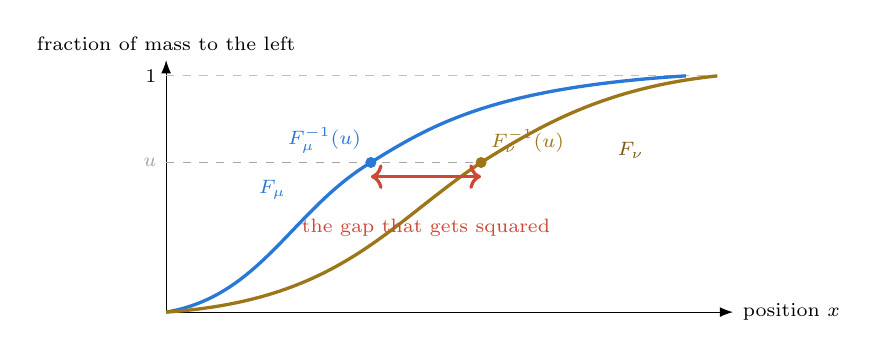
\begin{tikzpicture}[scale=1.0, every node/.style={font=\scriptsize}]
\draw[-Latex] (0,0) -- (7.2,0) node[right]{position $x$};
\draw[-Latex] (0,0) -- (0,3.2) node[above]{fraction of mass to the left};
\node[left] at (0,3.0) {$1$};
\draw[gray!50, dashed] (0,3.0) -- (7,3.0);
% CDF mu
\draw[intu, very thick] (0,0) .. controls (1.2,0.2) and (1.6,1.3) .. (2.6,1.9)
  .. controls (3.4,2.4) and (4.2,2.85) .. (6.6,3.0);
\node[intu] at (1.35,1.55) {$F_\mu$};
% CDF nu (shifted right)
\draw[golden!80!black, very thick] (0,0) .. controls (2.2,0.15) and (2.8,1.1) .. (4.0,1.9)
  .. controls (4.8,2.4) and (5.6,2.85) .. (7.0,3.0);
\node[golden!60!black] at (5.9,2.05) {$F_\nu$};
% level u, horizontal gap
\draw[gray!70, dashed] (0,1.9) node[left]{$u$} -- (4.0,1.9);
\fill[intu] (2.6,1.9) circle (2pt) node[above left]{$F_\mu^{-1}(u)$};
\fill[golden!80!black] (4.0,1.9) circle (2pt) node[above right]{$F_\nu^{-1}(u)$};
\draw[<->, very thick, warn] (2.6,1.72) -- (4.0,1.72);
\node[warn, below] at (3.3,1.30) {the gap that gets squared};
\end{tikzpicture}

{\scriptsize\emph{Legend: each curve climbs from 0 to 1 as it sweeps left to
right, accumulating its pile's mass (blue $=$ pile $\mu$, yellow $=$ pile
$\nu$). Pick any mass level $u$ (dashed): the \textbf{horizontal} gap between
the curves at that level is how far the $u$-th ``slice'' of sand must travel.
$W_2^2$ is the average of that squared gap over all levels $u \in [0,1]$ ---
Equation~\eqref{eq:quantile} is literally this picture, integrated.}}
\end{center}

Our soil bed, summarized as \emph{mass per vertical column} over the horizontal
axis (64 bins), is exactly such a 1D distribution, and soil mass is conserved
during an episode --- so this formula gives us the \textbf{true physical
transport cost between any two soil states, thousands of times per second,
during training}. (For genuinely 2D mass fields there is \emph{sliced} $W_2$:
average the 1D formula over many random projection directions. We use it in
Experiment 5.)

% ============================================================
\section{Our method: TMSD}
% ============================================================

\subsection{The two ingredients}

Take METRA's template \eqref{eq:metra} and change two things:

\textbf{Ingredient 1 — a physical ground metric.} Let $\mu_s$ denote the soil
mass distribution in state $s$, and set
\[
d(s, s') \;=\; W_2(\mu_s, \mu_{s'}).
\]
The Lipschitz constraint becomes: \emph{one unit of latent motion must be backed
by one unit of physical mass transport} (tons moved $\times$ meters). Skills, to
earn reward, must differ by how they \emph{move soil}.

\textbf{Ingredient 2 — external-state conditioning.} The representation $\phi$
receives \textbf{only} the soil measure $\mu$ --- never a joint angle, never a
velocity. Then for any behavior that only moves the arm, $\phi(\mu') = \phi(\mu)$
and the reward is \emph{exactly zero by construction}. Arm-dancing is not
discouraged; it is \textbf{unpaid}.

The full objective:
\begin{equation}
\max_{\pi, \phi} \; \mathbb{E}\big[(\phi(\mu_{t+1}) - \phi(\mu_t))^{\!\top} z\big]
\quad \text{s.t.} \quad
\|\phi(\mu) - \phi(\mu')\| \le W_2(\mu, \mu'),
\label{eq:tmsd}
\end{equation}
optimized with the Lagrangian dual described earlier (with a \emph{relative}
slack cap, because $W_2$ steps span orders of magnitude, unlike METRA's constant
temporal distance), and SAC underneath. The intrinsic reward is recomputed with
the \emph{current} $\phi$ at every gradient step, since $\phi$ keeps improving
and stale rewards would anchor the policy to an obsolete map.

\subsection{What we believed, and what we pre-registered}
Going in, we believed Ingredient 1 (the transport metric) was the scientific
contribution and Ingredient 2 was plumbing. Following good practice, we
pre-registered the ablation that could falsify this (swap $W_2$ for Euclidean
and temporal metrics) \emph{and} the pivot rule if it failed. It failed. The
report below is the honest record --- and the replacement finding is stronger
than the original bet.

\subsection{The testbed}
Custom 2D discrete-element (DEM) simulation: $\sim$1200 circular soil grains
with Hertzian contact forces, Coulomb friction, rolling resistance and cohesion;
a three-joint (boom/stick/bucket) hydraulic arm with realistic torque and speed
limits, base fixed at $x{=}2$\,m in a 12.8\,m domain; CUDA-accelerated. Agent
observation (35-dim): joint angles/velocities, wrist pose, contact forces,
payload mass, 16-bin soil heightfield. Action (3-dim): joint velocity commands.
The soil measure $\mu$ for $\phi$: a 64-bin, mass-weighted, normalized histogram
over $x$. Skills: $z$ uniform on the unit sphere in $\mathbb{R}^4$. Episodes:
200 steps. All methods trained with identical budgets (200k environment steps
$=$ 200k gradient updates, $\sim$1.5--2.5\,h per run on one RTX 5080).

\subsection{How the state is represented: four layers}

It is worth being very explicit about \emph{who sees what}, because the
project's central finding lives entirely in this split.
Figure~\ref{fig:representation} shows all four layers for one real state:

\begin{enumerate}[leftmargin=6mm]
\item \textbf{Ground truth} (simulation only): $\sim$1200 particles $\times$
(position, velocity, radius, mass) plus the arm --- thousands of dimensions
nobody observes directly.
\item \textbf{The policy's observation} (35 numbers): joint angles and
velocities, wrist pose, contact forces, payload, and a coarse 16-bin soil
heightfield. The \emph{policy} is allowed to know its own body --- it needs to,
to control it.
\item \textbf{The external measure $\mu$} (64 numbers): soil mass per column,
normalized to sum to 1, \emph{zero robot information}. This --- and only this ---
is what the objective's representation $\phi$ ever receives. Note the asymmetry
with layer 2: the policy's soil view is a coarse \emph{height} field; $\phi$'s is
a finer \emph{mass} distribution --- the physically meaningful object for
transport.
\item \textbf{The latent $\phi(\mu) \in \mathbb{R}^4$}: a small MLP trained
under the Lipschitz constraint. Skills are directions here, goals are points
here, and steering is arithmetic here.
\end{enumerate}

\begin{figure}[h]
\centering
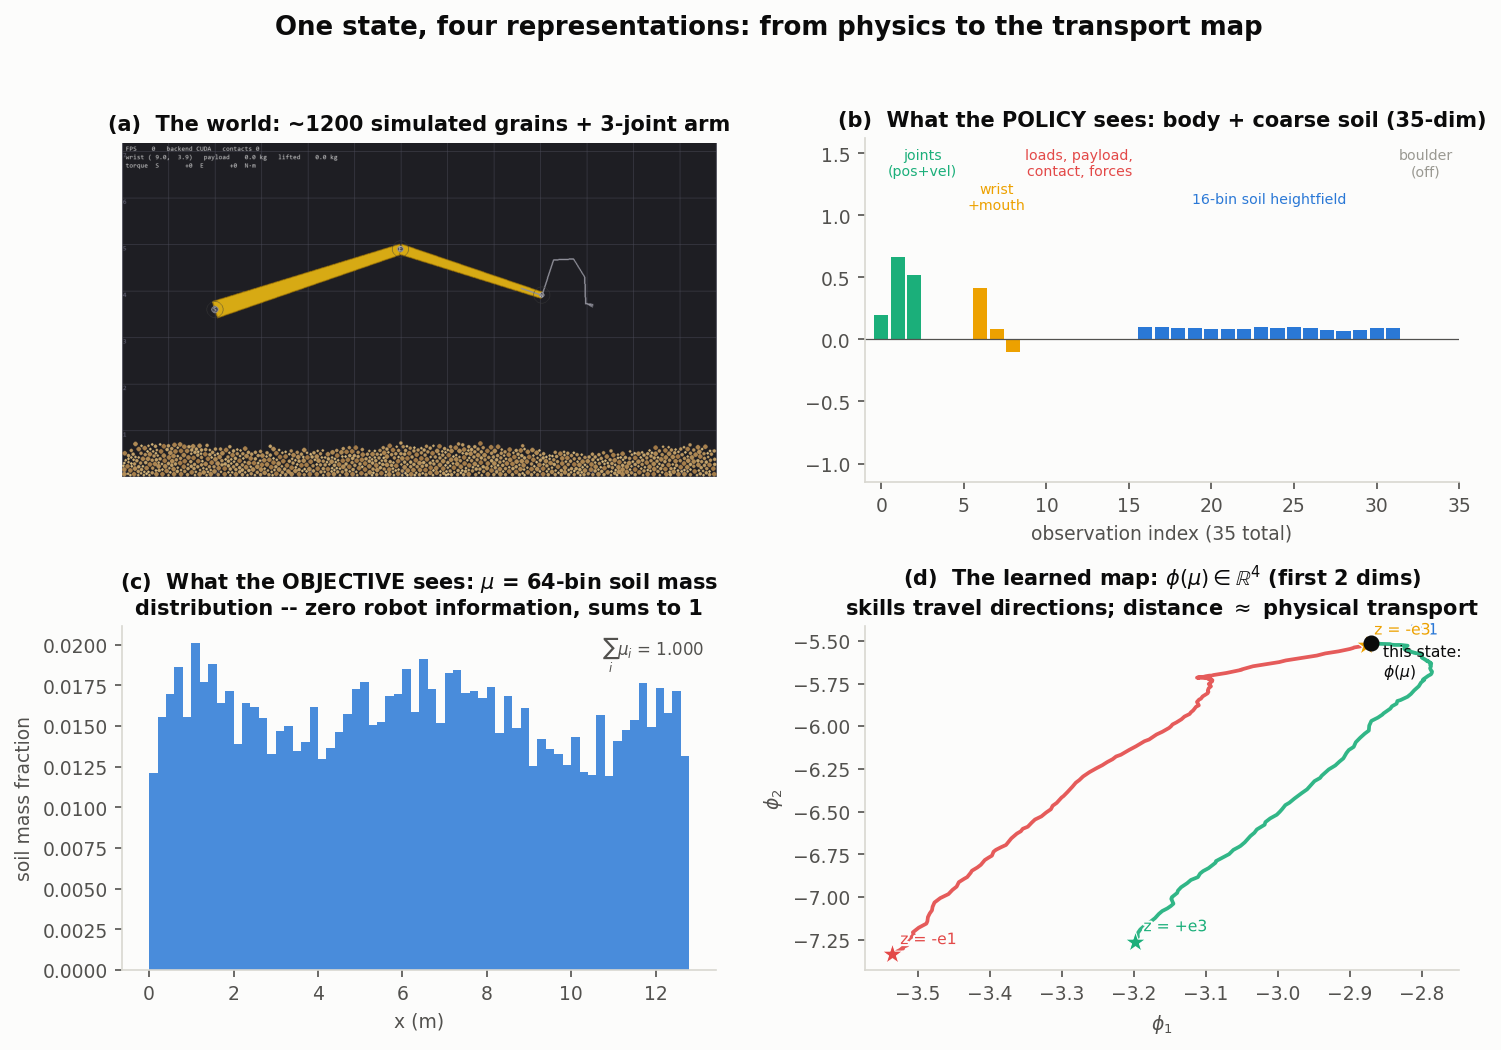
\includegraphics[width=0.98\linewidth]{fig_representation.png}
\caption{One state, four representations, all real data through the trained
model. (a)~the simulated world; (b)~the 35 numbers the policy acts on,
color-grouped; (c)~the soil mass distribution $\mu$ --- the objective's entire
universe, summing to exactly 1; (d)~the state's position on the learned latent
map, with four skill episodes traced for context (star $=$ terminal). Note in
(d) that one direction ($+e_1$) barely moves from the start: a \emph{dead
direction} on this terrain, honestly visible.}
\label{fig:representation}
\end{figure}

% ============================================================
\section{The experiments}
% ============================================================

Each experiment follows the same template: \emph{the problem} it answers,
\emph{the test}, \emph{the result} (with the actual data), and \emph{the
insight} that determined what we did next.

% ------------------------------------------------------------
\subsection{Experiment 1 — Does anything emerge at all?}

\textbf{Problem.} No one has run USD on granular media. Perhaps nothing happens:
contact-rich digging is hard even for rewarded RL.

\textbf{Test.} TMSD as in \eqref{eq:tmsd}, 500k steps, fixed initial terrain,
skill dimension 2 (a pilot: small and interpretable).

\begin{figure}[h]
\centering
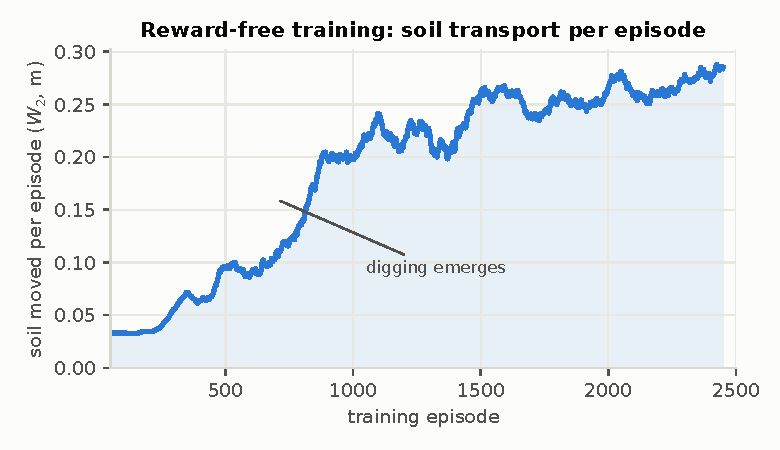
\includegraphics[width=0.62\linewidth]{fig_learning_curve.pdf}
\caption{Soil transported per episode ($W_2$ between the episode's initial and
final soil states) over reward-free training. Rolling mean over 100 episodes.
The rise from $\approx 0.03$\,m (ambient settling --- what the soil does with a
motionless arm) to $\approx 0.28$\,m is digging being \emph{invented}.}
\label{fig:learning}
\end{figure}

\textbf{Result.} Skills emerge that \emph{dig}: scoop into the bed, drag material,
build spoil piles --- reward-free. By late training the policy moves nearly
$10\times$ the ambient soil motion per episode.

\begin{figure}[h]
\centering
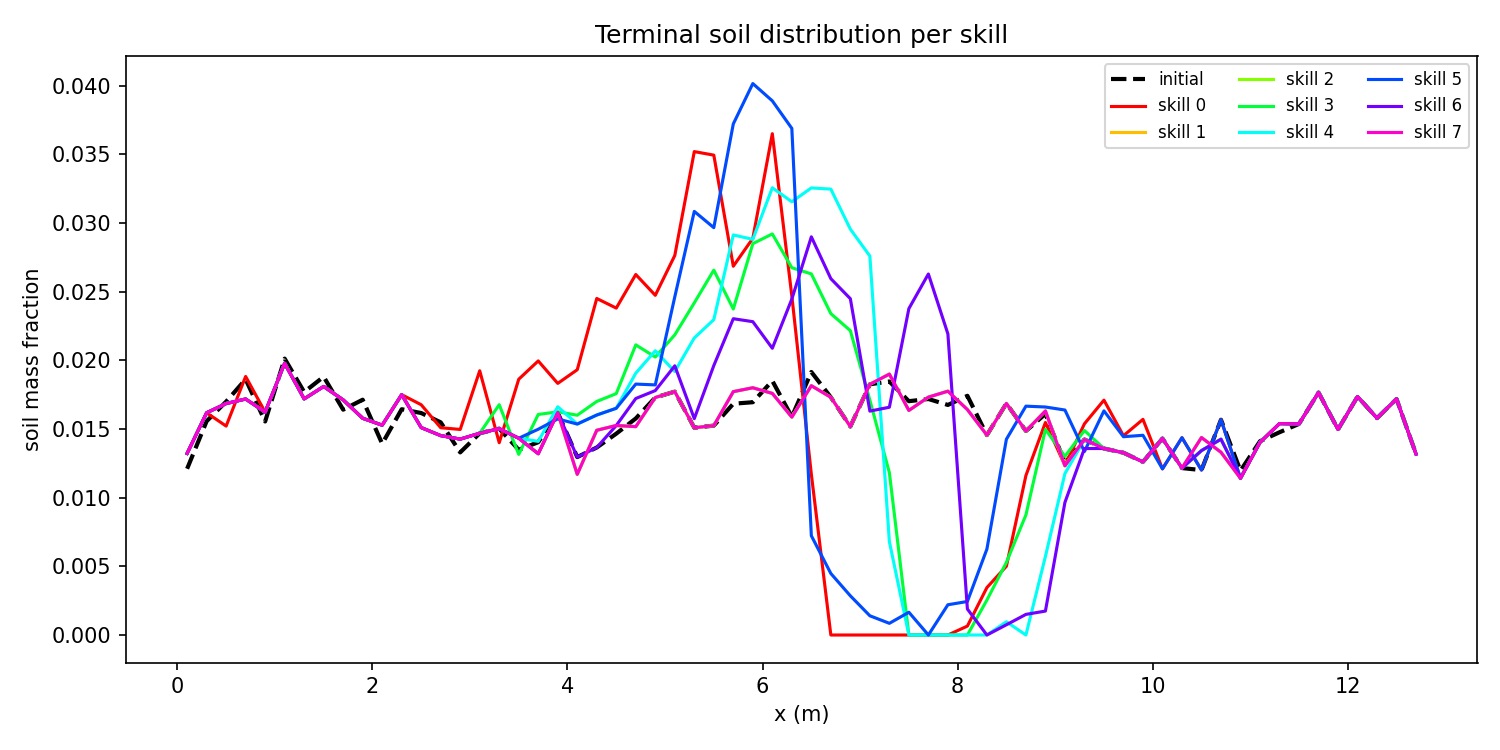
\includegraphics[width=0.56\linewidth]{fig_terminal_profiles.png}%
\hfill
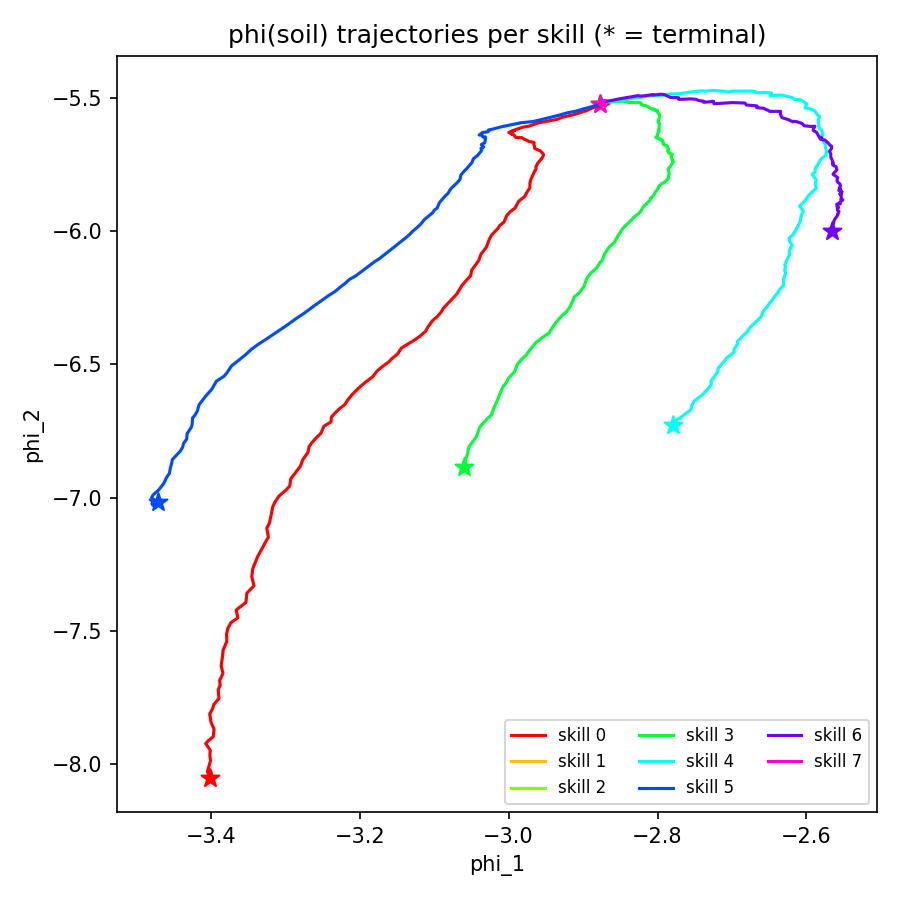
\includegraphics[width=0.42\linewidth]{fig_phi_trajectories.png}
\caption{\textbf{Left:} terminal soil profiles for 8 skill directions vs.\ the
initial terrain (dashed): different skills excavate and deposit at different
locations. \textbf{Right:} the latent representation at work --- each curve is
$\phi(\mu_t)$ over one episode, colored by skill ($\star$ = terminal). The fan
structure is the objective \eqref{eq:tmsd} realized: each skill travels its own
latent direction, and by the constraint, latent distance $\approx$ physical
transport. This latent space is the robot's learned ``map of soil states.''}
\label{fig:profiles}
\end{figure}

\textbf{Insight.} The skill coordinate is physically interpretable: the sign of
$z_1$ equals the direction the soil's center of mass shifts (measured $\pm$0.10
to 0.16\,m per episode). One caveat appeared: with the fixed terrain and
$\dim z = 2$, only $\approx 3$ genuinely distinct behaviors emerged (hold /
push-left / push-right around one spot) --- the latent capacity bounds how many
physical axes the skills can span. This motivated $\dim z = 4$ plus terrain
randomization (a random smooth height envelope per episode) for every subsequent
experiment.

% ------------------------------------------------------------
\subsection{Experiment 2 — Is the transport metric doing the work?}
\label{sec:metricablation}

\textbf{Problem.} Our headline hypothesis. If $W_2$ is the load-bearing
ingredient, replacing it should hurt.

\textbf{Test.} Identical recipe, three seeds each, swapping only $d$ in the
constraint of \eqref{eq:tmsd}: (a) $W_2$ (ours); (b) \emph{Euclidean} distance
between the 64-bin histograms (geometry-blind); (c) \emph{temporal} $d \equiv 1$
(METRA's original). All evaluated by one frozen protocol: coverage $=$ mean
pairwise $W_2$ between terminal soil states over 8 fixed skills $\times$ 3 fixed
terrains (the protocol was frozen \emph{before} results were seen, so the ruler
could not be chosen to flatter anyone).

\textbf{Result.}
\begin{center}
\begin{tabular}{lccc}
\toprule
ground metric & $W_2$ (ours) & Euclidean & temporal (METRA)\\
\midrule
coverage (m), 3 seeds & $0.326 \pm 0.029$ & $0.351 \pm 0.030$ & $0.290 \pm 0.077$\\
\bottomrule
\end{tabular}
\end{center}
A three-way statistical tie. \textbf{Our hypothesis is falsified.}

\textbf{Insight --- why the metric cannot matter here.} We measured, for every
trained model, the correlation between latent distance $\|\phi(\mu_a) -
\phi(\mu_b)\|$ and physical $W_2(\mu_a, \mu_b)$ over thousands of visited state
pairs. \emph{Every} model --- including those trained with the Euclidean and
temporal constraints --- came out at $\approx 0.99$ (Pearson and Spearman). The
latent maps all became near-isometries of the physical transport geometry
\textbf{without being asked}. Explanation: the set of soil states reachable in a
200-step episode is effectively low-dimensional (dig more/less, left/right,
near/far). Along such a thin manifold, all reasonable metrics are monotone
re-parameterizations of one another --- they can only disagree on state pairs
the policy never visits. \emph{Geometry is emergent and free; the metric choice
is not where the leverage is.}

% ------------------------------------------------------------
\subsection{Experiment 3 — Then what IS doing the work?}
\label{sec:factorization}

\textbf{Problem.} If not the metric, perhaps the conditioning: $\phi$ seeing
only soil.

\textbf{Test.} Identical run, but $\phi$ receives the \emph{full} 35-dim
observation (proprioception $+$ soil). This is precisely vanilla METRA. Three
seeds.

\begin{figure}[h]
\centering
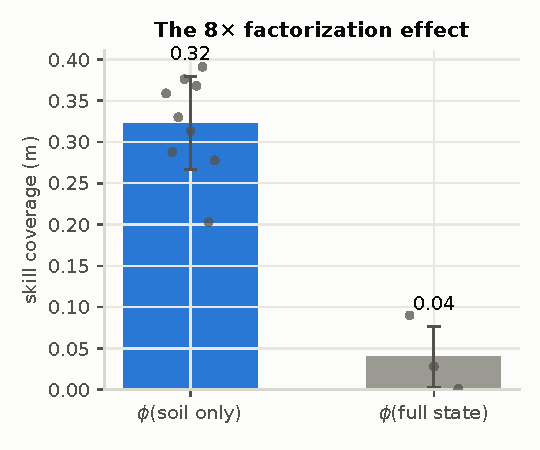
\includegraphics[width=0.4\linewidth]{fig_factorization.pdf}%
\hspace{6mm}%
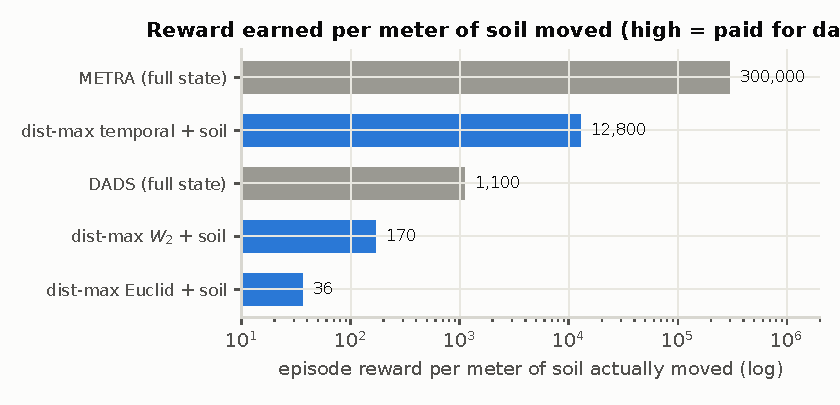
\includegraphics[width=0.52\linewidth]{fig_reward_per_meter.pdf}
\caption{\textbf{Left:} the factorization effect --- dots are individual runs
(9 soil-conditioned across all metrics; 3 full-state). \textbf{Right:} reward
collected per meter of soil actually moved (log scale): a ``lie detector'' for
objectives. Full-state models earn $\sim$300{,}000 reward-units per meter ---
they are being paid for something other than soil. The $W_2$-constrained model's
$\sim$170 is the honest number: its rewards are denominated in physical
transport.}
\label{fig:factor}
\end{figure}

\textbf{Result.} Coverage $0.323 \pm 0.028$ (soil-only, pooled over metrics,
9 runs) vs.\ $0.039 \pm 0.036$ (full-state, 3 runs): an \textbf{8$\times$
effect}, and the full-state failure is qualitative --- 7 of 8 skills never touch
the soil. Watching it is comic: the arm performs elaborate, skill-distinct
choreography above an untouched bed.

\textbf{Insight.} \emph{What you show the discriminator determines what the
skills are about.} The ingredient we had treated as plumbing is the load-bearing
wall. This reframing --- the discriminator's input as a \textbf{task-specification
language} (``point the objective's attention at the subsystem you care about'') ---
became the project's central claim.

% ------------------------------------------------------------
\subsection{Experiment 4 — The metric's second chance (2D measure)}

\textbf{Problem.} Maybe Experiment 2's tie was an artifact of the crude 1D
measure: a deep narrow hole and a wide shallow one have identical column sums,
so \emph{no} 1D metric can tell them apart. On a full 2D mass grid
($48 \times 24$ bins over $x,y$), transport structure could finally matter.

\textbf{Test.} Rerun the metric ablation with 2D measures: sliced-$W_2$
(Section~\ref{sec:1dw2}) vs.\ Euclidean vs.\ temporal, same recipe.

\textbf{Result.} Sliced-$W_2$ coverage: $0.044$. Euclidean-2D: $0.245$.
Temporal-2D: $0.214$. The transport metric is not merely unhelpful here ---
it is \textbf{5$\times$ worse, on its own preferred yardstick}.

\textbf{Insight (from training telemetry, not speculation).} Under the SW$_2$
constraint the representation extracted only $\sim$7\% of the reward its
constraint budget allowed (the Euclidean control: $\sim$45\%). The reward signal
never grew teeth; the policy never received a usable gradient; behavior stayed at
ambient. Mechanism: \emph{optimization starvation}, not mis-valued behavior. The
honest summary of Experiments 2$+$4: \textbf{the physical transport metric is
conclusively not the source of skill diversity --- in the rich regime it can even
prevent learning.} What survives of $W_2$: rewards with physical units (meters of
mass transport), i.e.\ \emph{calibration}, useful for the goal-reaching layer
below.

% ------------------------------------------------------------
\subsection{Experiment 5 — Composing skills into goals (zero-shot shaping)}
\label{sec:goal}

\textbf{Problem.} Diverse skills are means, not ends. Can they be \emph{aimed}?
Given a target soil profile $\mu^\ast$ (a trench, a berm), can the trained system
reach it with \textbf{no further training}?

\textbf{Test.} The zero-shot steering rule: every 10 steps, command the skill
\[
z \;=\; \frac{\phi(\mu^\ast) - \phi(\mu_{\text{now}})}{\|\phi(\mu^\ast) - \phi(\mu_{\text{now}})\|}
\]
--- literally ``point the skill-knob at the goal's location on the latent map.''
This works only if the latent map is geometrically faithful (which
Experiment~2's isometry result guarantees).

\begin{figure}[h]
\centering
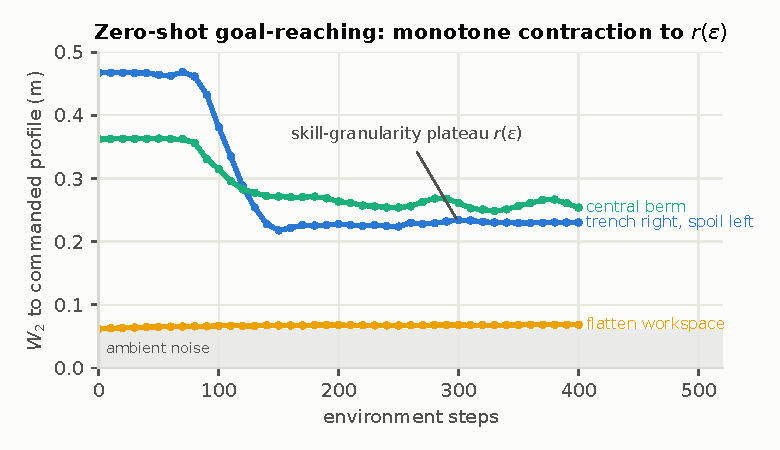
\includegraphics[width=0.6\linewidth]{fig_contraction.pdf}
\caption{$W_2$-to-goal during zero-shot steering, three commanded targets. The
trench command halves the distance ($+51\%$); the berm $+28\%$; the ``flatten''
target starts \emph{below} the resolvable scale and correctly does almost
nothing. Note the plateau: contraction stops at $r(\varepsilon) \approx
0.2$\,m --- the \emph{skill granularity radius}.}
\label{fig:contraction}
\end{figure}

\textbf{Result.} Across 21 targets and 9 checkpoints: \textbf{39--63\% of the
distance to goal removed, zero-shot}; 79--94\% of control intervals decrease
$W_2$ \emph{monotonically} --- an empirical \emph{contraction certificate}
(each skill application provably-in-practice brings the soil closer). In the
executable demo, the order ``excavate $x \in [7,9]$, dump at $x \in
[4.5,6.5]$'' removes \textbf{79\% of the dig zone's soil} and fills the dump
zone to within 2.6 points of target (Figure~\ref{fig:demo}).

\begin{center}
\small
\begin{tabular}{lccc}
\toprule
model (seed) & goal improvement & monotone intervals & latent--physical corr.\\
\midrule
$W_2$ (s0 / s1 / s2) & $58 / 45 / 39\,\%$ & $91 / 82 / 84\,\%$ & $0.99 / 0.99 / 0.99$\\
Euclid (s0 / s1 / s2) & $63 / 54 / 47\,\%$ & $94 / 91 / 79\,\%$ & $0.99 / 0.99 / 0.99$\\
temporal (s0 / s1 / s2) & $63 / 44 / 54\,\%$ & $92 / 85 / 91\,\%$ & $0.99 / 0.98 / 0.98$\\
\bottomrule
\end{tabular}
\end{center}

\noindent The last column is Experiment 2's isometry result, per seed: every
latent map, whatever its training metric, measures physical transport at
correlation $\approx 0.99$ --- which is precisely why pointing $z$ at the goal's
latent works for all of them, and why none of them steers better than another.

\textbf{Insight.} The plateau $r(\varepsilon)$ is not noise --- it is the
theoretically expected residual: skills $\varepsilon$-cover the directions of
transport, so greedy composition contracts until goals are finer than the
coarsest available move, then stalls. This number returns, decisively, in
Experiment~8.

\begin{figure}[p]
\centering
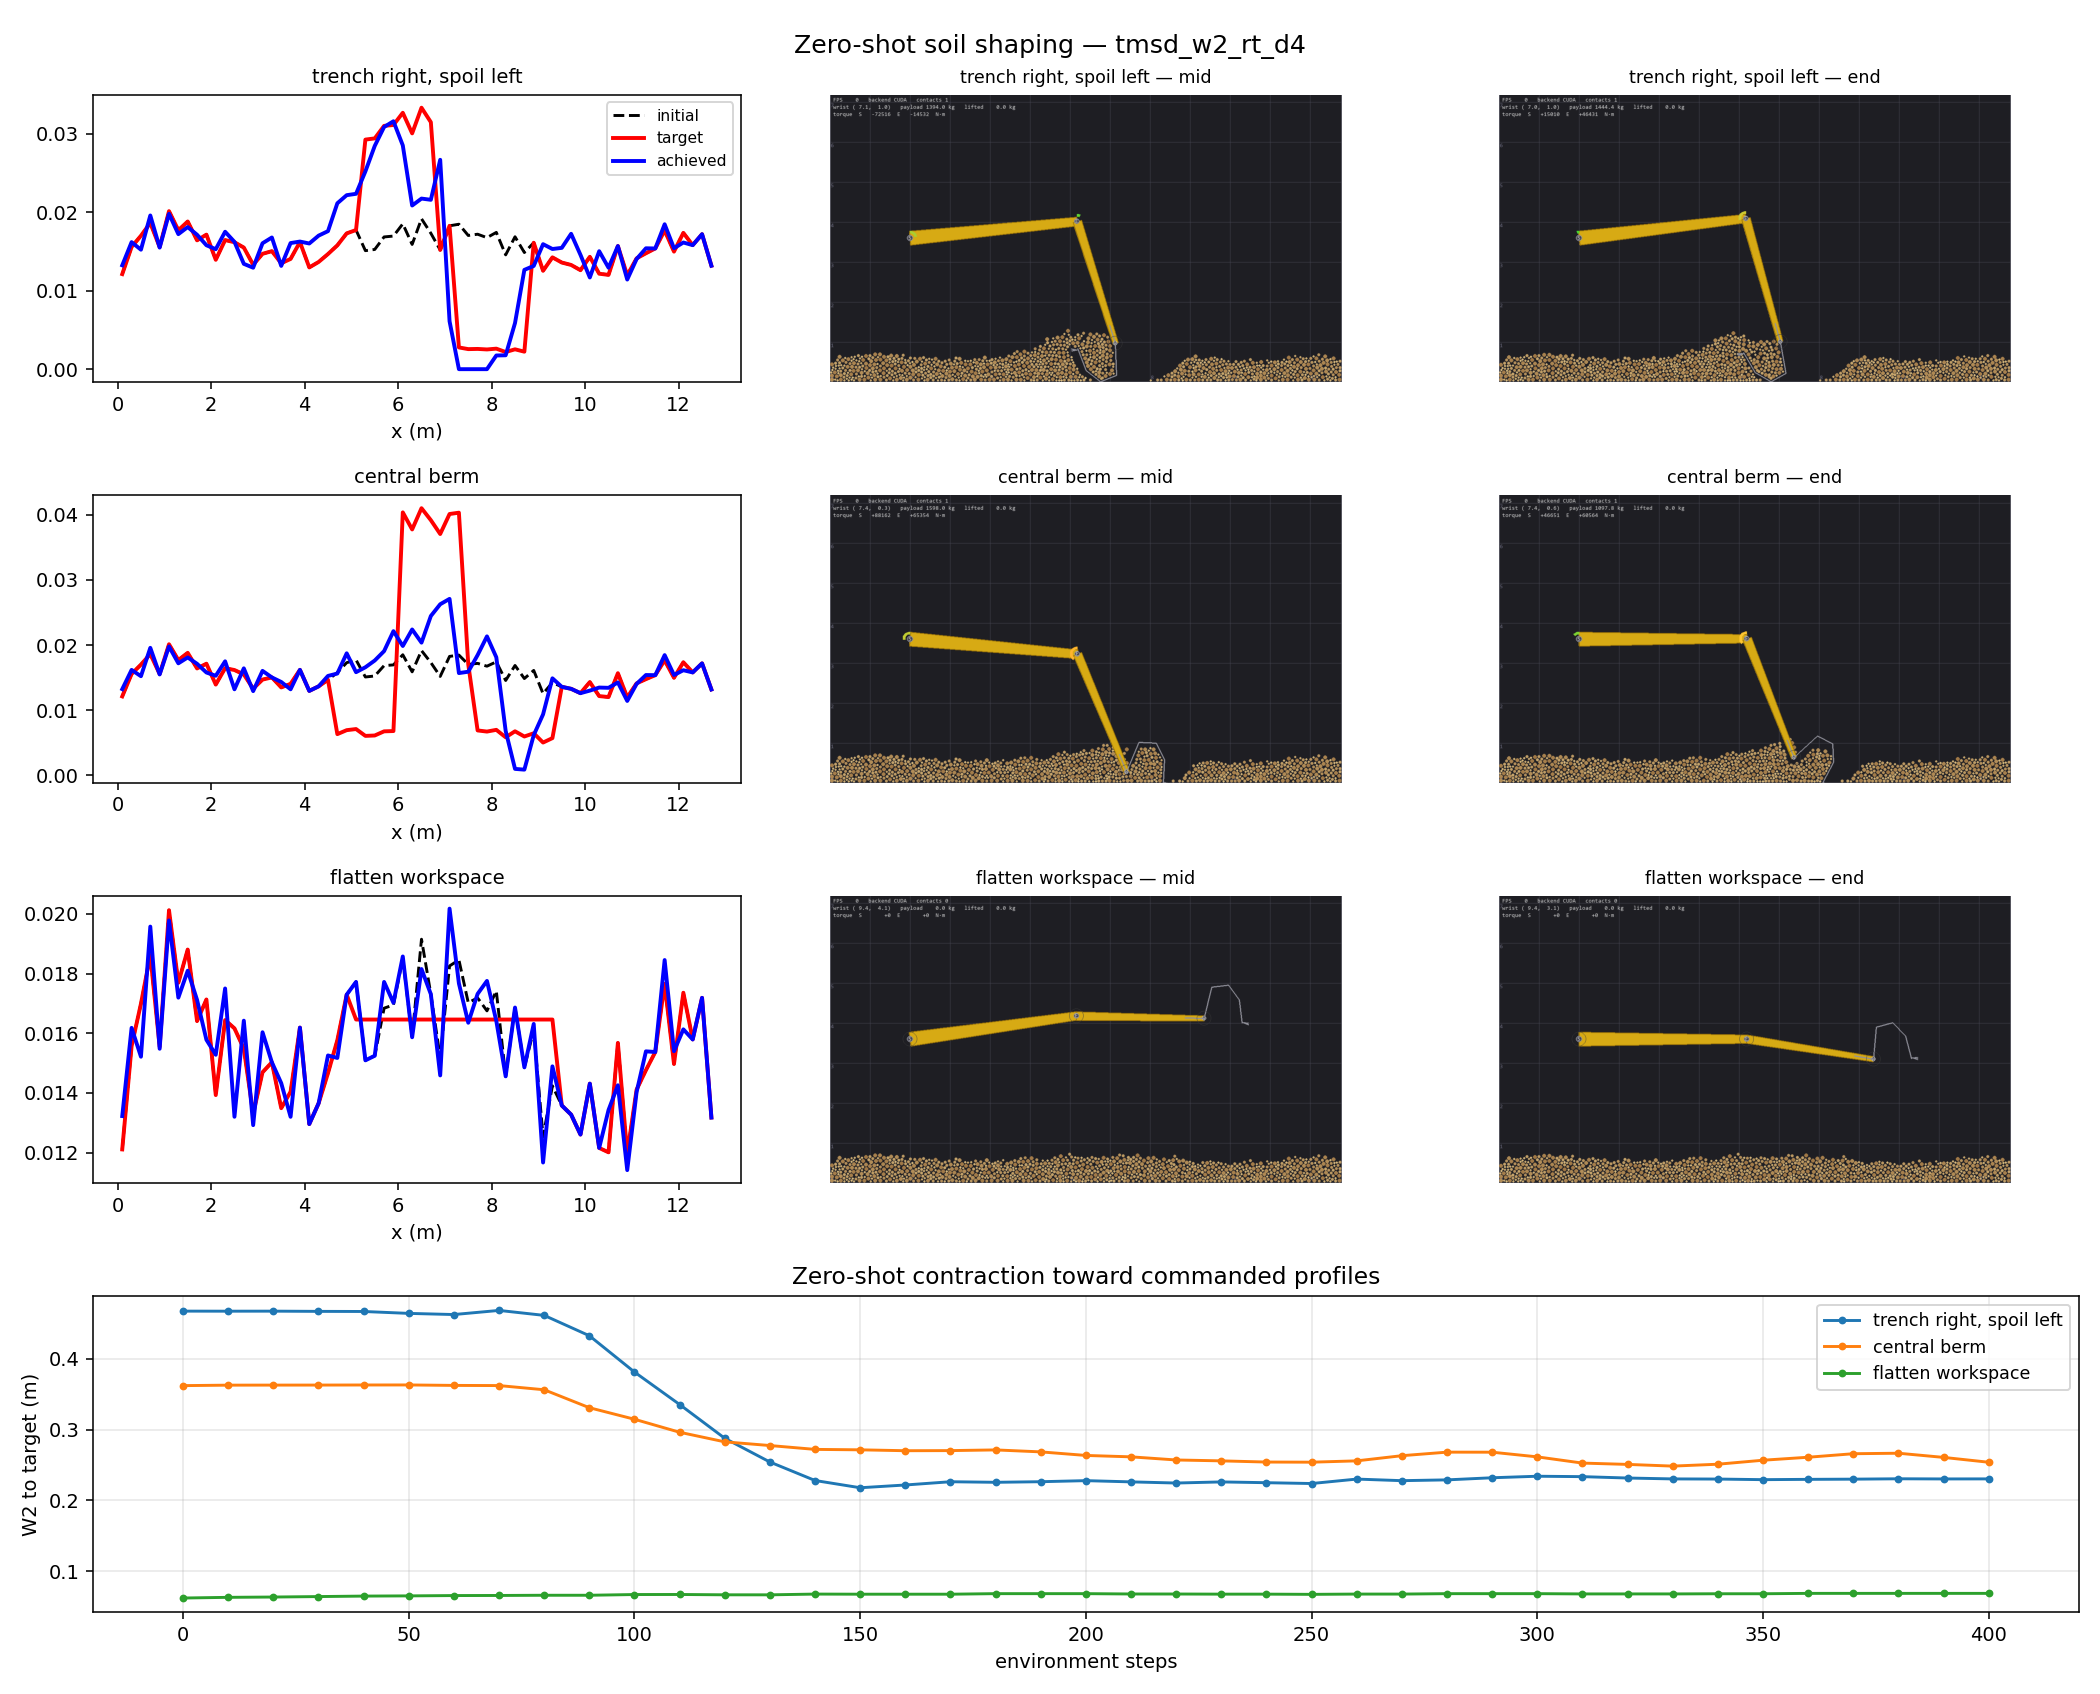
\includegraphics[width=0.94\linewidth]{fig_demo_shaping.png}
\caption{The zero-shot shaping demo in full: per-target profiles (initial /
target / achieved), simulator frames mid- and end-execution, and the contraction
curves. No reward, no planner, no goal-conditioned training --- composition of
reward-free skills via latent steering.}
\label{fig:demo}
\end{figure}

% ------------------------------------------------------------
\subsection{Experiment 6 — DIAYN on soil (the MI $2\times2$)}
\label{sec:mi2x2}

\textbf{Problem.} Is external conditioning \emph{alone} sufficient? Then an
MI objective with soil-only inputs should also work.

\textbf{Test.} Continuous-DIAYN (discriminator predicts $z$ from the state;
reward $=$ cosine agreement), crossed with both conditionings, 3 seeds per cell,
identical recipe.

\textbf{Result.} Both MI cells fail: coverage $0.021 \pm 0.015$ (soil-only) and
$0.031 \pm 0.028$ (full-state) --- ambient. The mechanism is visible in training
curves (Figure~\ref{fig:mechanisms}, middle): the discriminator reaches $0.98$
cosine accuracy \emph{almost immediately} --- microscopic, static grain
differences suffice to identify the skill --- and thereafter nothing demands
further change. \textbf{Saturation}, exactly as the theory of
Section~4.1 predicts, now measured on a material.

\textbf{Insight.} Conditioning is necessary but \emph{not} sufficient. The
objective family matters too --- MI-style identifiability cannot power material
manipulation.

% ------------------------------------------------------------
\subsection{Experiment 7 — DADS on soil}

\textbf{Test.} Faithful DADS (skill-dynamics model $+$ predictability-advantage
reward, $L{=}16$ alternatives), both conditionings, 2 seeds per cell.

\textbf{Result.} Soil-conditioned DADS: coverage $0.008 \pm 0.008$ ---
statistically zero --- with per-step reward measured at \textbf{0.000 for the
entire run} (Figure~\ref{fig:mechanisms}, bottom). \textbf{Starvation},
exactly as Section~4.2 predicts: soil's per-step deltas are almost always nil,
hence equally predictable under every skill, hence zero advantage. Full-state
DADS: $0.130 \pm 0.073$ --- one seed reached $0.203$ through arm-dynamics skills
that \emph{incidentally} contact the bed (its sibling seed: $0.057$); highest
variance in the study and still $2.5\times$ below the working family.

\begin{figure}[h]
\centering
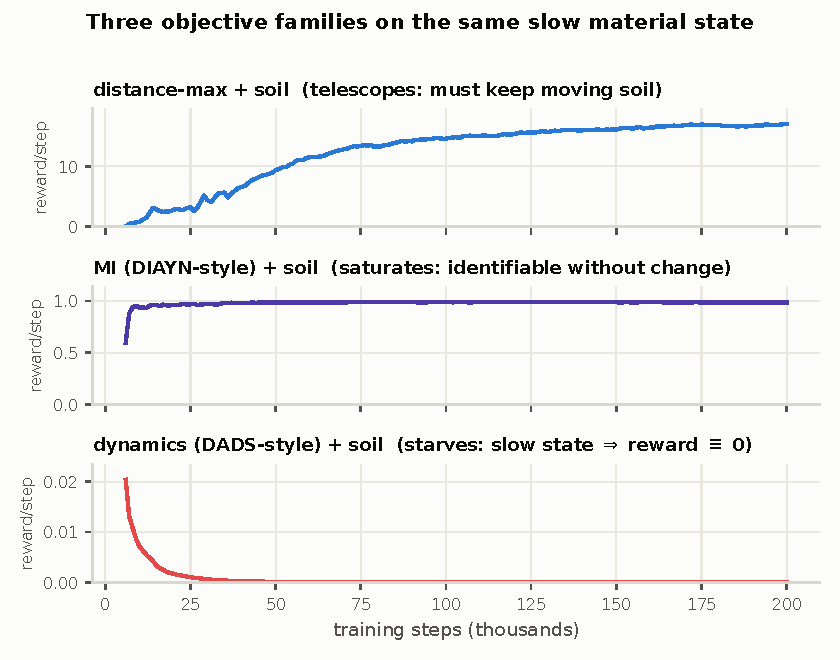
\includegraphics[width=0.62\linewidth]{fig_mechanisms.pdf}
\caption{The three objective families' intrinsic reward over training, all with
soil-only conditioning, all on the same simulator. Top: distance-maximizing ---
reward \emph{grows} as digging improves (it telescopes; only net transport
pays). Middle: MI --- \emph{saturates} within a few thousand steps and flatlines.
Bottom: dynamics-predictability --- \emph{starves} to exactly zero. This single
figure is the taxonomy.}
\label{fig:mechanisms}
\end{figure}

% ------------------------------------------------------------
\subsection{The unifying law: materials are slow states}

Soil changes rarely and gradually; the arm changes richly at every step. Write
each objective's reward as a function of the state sequence and this one
property sorts everything:

\begin{itemize}[leftmargin=6mm]
\item \textbf{MI (DIAYN):} pays for per-step \emph{identifiability}. Slow states
still carry stable microscopic fingerprints $\Rightarrow$ maximal reward without
macroscopic change $\Rightarrow$ \textbf{saturates}.
\item \textbf{Dynamics (DADS):} pays for per-step \emph{predictability
advantage}. Slow states are trivially predictable under all skills
$\Rightarrow$ the advantage is identically zero $\Rightarrow$ \textbf{starves}.
\item \textbf{Distance-max (METRA family):} by the telescoping identity
\eqref{eq:telescope}, pays for \emph{net cumulative displacement} of the
(soil) state $\Rightarrow$ the only reward that a slow state can still feed,
because it \emph{integrates} change over the episode instead of grading it per
step $\Rightarrow$ \textbf{works}.
\end{itemize}

\begin{keyresult}[title=\textbf{The two-ingredient design law}]
On slow external states (materials), a skill-discovery objective must
\textbf{(i)} integrate change over time rather than score it per step
(distance-maximizing / telescoping structure), and \textbf{(ii)} be conditioned
\emph{only} on the external state. In our $3\times2$ grid (three objective
families $\times$ two conditionings, 2--3 seeds per cell), exactly the one cell
with both properties works --- at $8\times$ the coverage of the best cell
lacking either.
\end{keyresult}

% ------------------------------------------------------------
\subsection{Experiment 8 — Where it honestly breaks (and why)}

\textbf{Problem.} An interactive demo: the user sculpts terrain with the mouse,
records it as a goal, wrecks it, and the excavator should restore it. It
performed poorly. Why?

\textbf{Diagnosis chain} (each hypothesis tested and dismissed in turn):
\begin{enumerate}[leftmargin=6mm]
\item \emph{Unfamiliar states?} We retrained \emph{on} user-like edits
(random push/remove/add operations at every reset). No improvement.
\item \emph{Poor skill selection?} We built a model-predictive controller that
uses \textbf{the simulator itself} as a perfect lookahead model: snapshot the
world, mentally roll out every candidate skill, execute the provably best one.
Improvement: $+6$--$13\%$ only.
\item With perfect selection eliminated, only one suspect remains: the
\textbf{vocabulary}. The discovered skills span 3--5 coarse global transport
modes; a freehand repair needs \emph{local} corrections at arbitrary positions
--- directions of state-space the diversity objective never valued, because they
contribute little diversity. Moreover user edits are typically \emph{smaller
than} $r(\varepsilon) \approx 0.2$\,m: inside the granularity radius where the
contraction certificate itself says progress stops.
\end{enumerate}

\begin{keyresult}[title=\textbf{Diversity $\neq$ controllability}]
Skill discovery optimizes for the few \emph{most mutually different} behaviors,
not for a dense basis of \emph{all} behaviors. It yields coarse reachability
of the state space --- ideal as pretraining and for coarse commanded work; below
its granularity radius, a task-optimized layer (e.g.\ goal-conditioned
fine-tuning warm-started from the skills) is required. $r(\varepsilon)$ makes
this boundary \emph{measurable}. A supporting negative: a goal-conditioned SAC
trained \emph{from scratch} (no skill pretraining) on the same tasks fails to
learn at all --- 800k steps of contact-rich exploration finding no gradient ---
evidence that the skills' role as \emph{initialization} is real.
\end{keyresult}

Two mechanical limits also surfaced, worth stating because they are physics, not
learning: (a) one bucket interaction disturbs $\sim$0.1\,m of $W_2$ --- repairs
smaller than a scoop are like surgery with a backhoe; (b) with a \emph{fixed}
base and backhoe geometry, soil transports only \emph{toward} the machine ---
real operators solve this by driving around the pile, and giving our machine a
mobile base is the corresponding fix.

% ------------------------------------------------------------
\subsection{The full frontier comparison}

\begin{figure}[h]
\centering
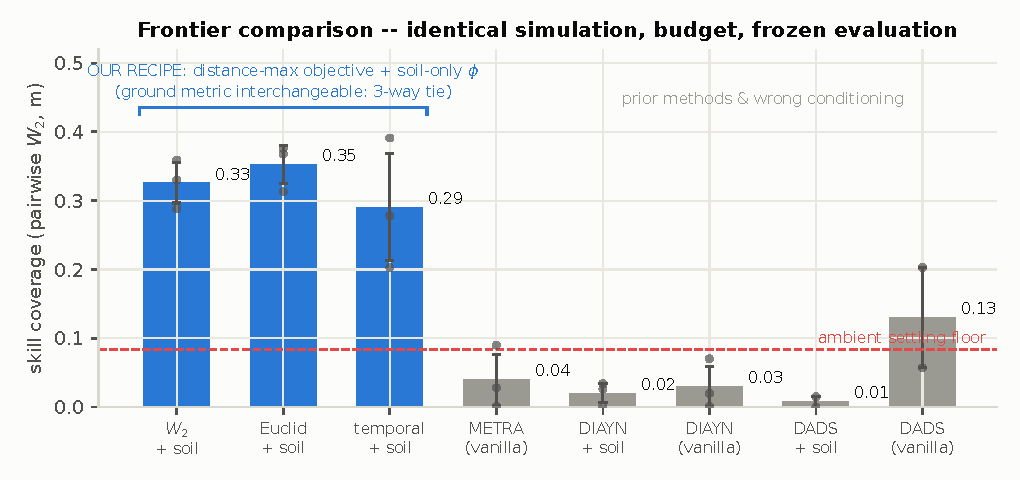
\includegraphics[width=0.9\linewidth]{fig_frontier_coverage.pdf}
\caption{Everything on one axis: 8 method-variants, identical simulation,
identical budget, frozen evaluation. Blue: distance-maximizing objectives with
soil-only conditioning (any metric). Gray: every other family and conditioning.
Dots are individual seeds; the dashed line is what soil does with a motionless
arm.}
\label{fig:frontier}
\end{figure}

\begin{table}[h]
\centering
\small
\begin{tabular}{llcc}
\toprule
\textbf{method} & \textbf{corresponds to} & \textbf{coverage (m)} & \textbf{seeds}\\
\midrule
dist-max $W_2$ + soil $\phi$ & ours (TMSD) & $0.326 \pm 0.029$ & 3\\
dist-max Euclidean + soil $\phi$ & ablation & $0.351 \pm 0.030$ & 3\\
dist-max temporal + soil $\phi$ & METRA + our conditioning & $0.290 \pm 0.077$ & 3\\
dist-max, full state & \textbf{vanilla METRA} & $0.039 \pm 0.036$ & 3\\
MI + soil $\phi$ & DIAYN + our conditioning & $0.021 \pm 0.015$ & 3\\
MI, full state & $\approx$ \textbf{vanilla DIAYN} & $0.031 \pm 0.028$ & 3\\
dynamics + soil $\phi$ & DADS + our conditioning & $0.008 \pm 0.008$ & 2\\
dynamics, full state & $\approx$ \textbf{vanilla DADS} & $0.130 \pm 0.073$ & 2\\
\midrule
sliced-$W_2$, 2D measure & ours (negative result) & $0.064$ & 1\\
\bottomrule
\end{tabular}
\caption{The frozen-protocol comparison. Every vanilla frontier method fails on
this domain; every distance-maximizing $+$ soil-conditioned variant succeeds;
metric choice within the working family is irrelevant. Configuration parity:
same networks ($\sim$315k parameters), optimizer, budget (200k steps), terrain
randomization, and evaluation; complete per-run data in
\texttt{runs/full\_comparison.csv}.}
\end{table}

\subsubsection*{How to read the next three figures (a plain-language decoder)}

The upcoming figures use four terms constantly. Here is each one, defined
without jargon, with the concrete objects behind them.

\paragraph{$\mu$ (``mu'') — the soil, written as a list of numbers.}
Chop the 12.8\,m soil bed into 64 vertical columns. Weigh the soil in each
column. Divide by the total, so the 64 numbers sum to 1. That list \emph{is}
$\mu$. Nothing more mysterious: $\mu = (0.011,\, 0.014,\, 0.017,\, \dots)$
means ``1.1\% of all the soil is in the leftmost column, 1.4\% in the next,
\dots''. Two different soil landscapes give two different lists. A number like
$W_2(\mu_a, \mu_b) = 0.3$\,m means: to physically rebuild landscape $a$ into
landscape $b$, a perfect bulldozer must move the soil, on average, 0.3 meters.
When any figure says ``coverage $= 0.386$\,m'', the unit is meters \emph{of
required earth-moving} --- a physical quantity, not an abstract score.

\paragraph{$\phi$ (``phi'') — the learned summary of $\mu$.}
$\phi$ is a small neural network. You feed it the 64 numbers of $\mu$; it
outputs just 4 numbers. Those 4 numbers are the state's \emph{coordinates on a
learned map} --- like reducing a whole country to a pin on a chart. The
training constraint forces this map to be honest: two soil states end up far
apart on the map \emph{only if} turning one into the other requires a lot of
real earth-moving. We call the map's output space the \textbf{latent space}
(``latent'' $=$ hidden/internal --- coordinates the network invented, not ones
we defined). When we plot ``$\phi_1$ vs $\phi_2$'' we are simply plotting the
first two of those 4 numbers.

\paragraph{Latent trajectory / latent spread.}
Run one episode: the soil changes step by step, so $\mu$ changes step by step,
so the pin $\phi(\mu)$ \emph{moves across the map}, tracing a curve --- the
\textbf{latent trajectory} of that episode. The \textbf{latent spread} of a
method is simply how far its 8 skills' curves fan out from the starting pin.
Crucial warning, and the point of Figure~\ref{fig:latentcmp}: a big fan is
meaningful \emph{only if the map is honest}. Vanilla METRA's map is calibrated
to time-steps, not to soil, so its skills draw a huge impressive fan while the
actual soil never changes --- a large map distance that corresponds to zero
earth moved. Always check the latent picture against the physical one.

\paragraph{The coverage matrix — all skill pairs, one grid.}
Take the 8 skills. Run each from the identical starting terrain; photograph the
final soil state of each ($\mu^{(1)}, \dots, \mu^{(8)}$). Now fill an
$8\times8$ grid: the cell in row $i$, column $j$ holds
$W_2(\mu^{(i)}, \mu^{(j)})$ --- the earth-moving distance between skill $i$'s
final world and skill $j$'s final world. Bright cell $=$ those two skills
genuinely did different things to the soil. Dark cell $=$ despite being
``different skills,'' they left the world in the same state. The diagonal is
always black (every skill matches itself). The \textbf{coverage score} quoted
everywhere in this report is just the average of all off-diagonal cells ---
``on average, how far apart are the worlds my skills produce?'' Reading
Figure~\ref{fig:covmats} with this key: our quilt of bright cells means
pairwise-distinct outcomes almost everywhere; METRA's single bright cross means
one skill did something and seven skills produced literally interchangeable
worlds; DIAYN's faint haze and DADS's black square mean nobody moved anything.

\subsubsection*{Inside the latent spaces: why the bars differ}

Numbers say \emph{that} the methods differ; Figure~\ref{fig:latentcmp} shows
\emph{why}, by opening each method's own latent space next to what its skills
physically accomplish --- same 8 skills, same terrain for every row. The single
most instructive quantity is the \textbf{scale of each latent map}:

\begin{center}
\small
\begin{tabular}{lccl}
\toprule
method & latent spread ($\phi$ units) & coverage (m) & reading\\
\midrule
METRA (vanilla) & $\sim$150 & 0.093 & huge fan of \emph{arm choreography}\\
\textbf{ours} & $\sim$2.5 & \textbf{0.386} & modest fan of \emph{soil transport}\\
DIAYN + soil & $\sim$0.002 & 0.036 & saturation jitter\\
DADS + soil & $\sim$0.00007 & 0.002 & starvation flatline\\
\bottomrule
\end{tabular}
\end{center}

Vanilla METRA's row is the arm-dancing indictment in one image: a textbook
eight-direction latent fan --- $60\times$ wider than ours --- above terminal
soil profiles that lie \emph{exactly on the initial terrain}. Its temporal
constraint grants $\sim$1 latent unit per time step \emph{regardless of what
changed}, so 200 steps of choreography buy a $\pm 150$ fan; latent diversity is
decoupled from the world. Ours is the only row where the two columns agree:
the $W_2$ cap makes every latent unit cost real mass transport, so a modest fan
\emph{means} five distinct excavations. Below, DIAYN's saturation and DADS's
starvation are visible as sheer magnitude: their latent spaces barely move at
all. The taxonomy of Section~7.8, readable as four axis scales.

\begin{figure}[p]
\centering
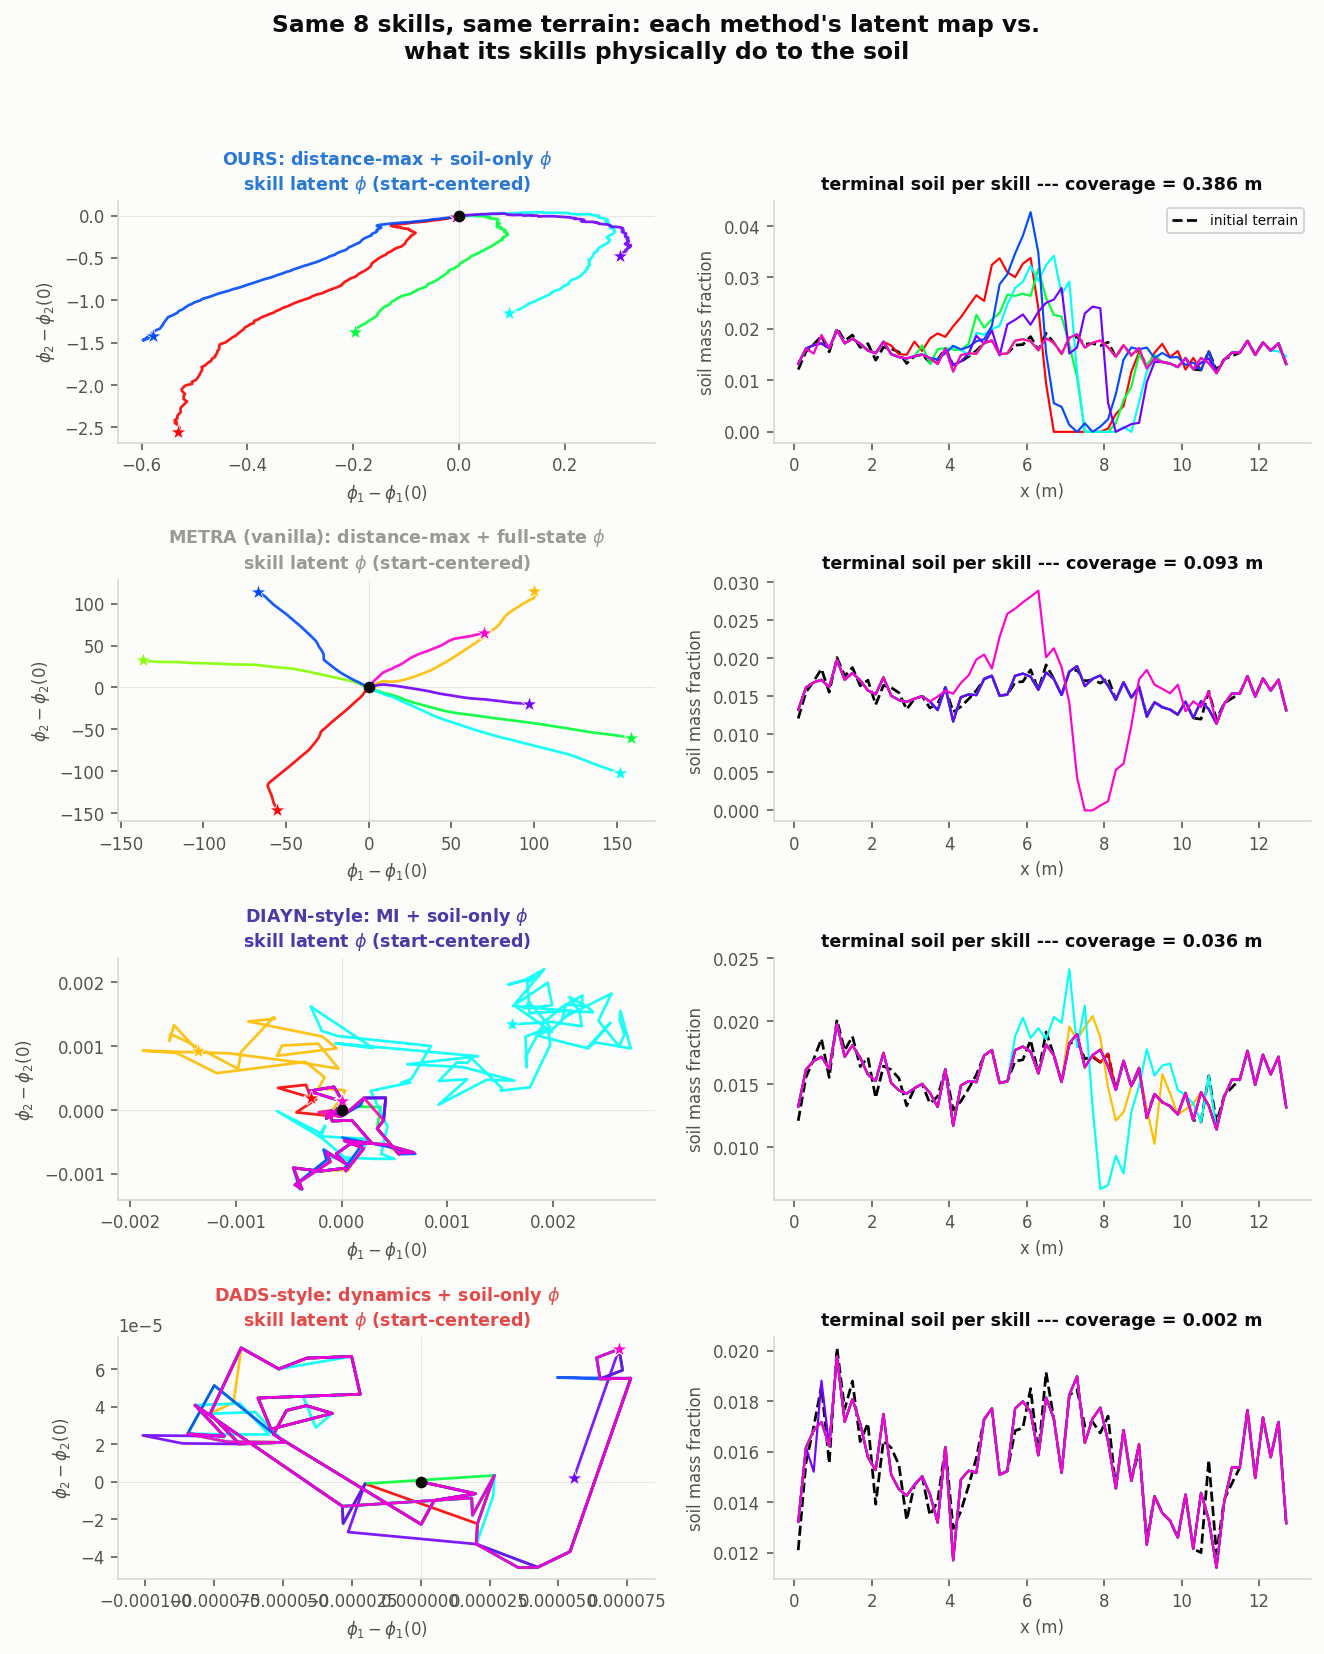
\includegraphics[width=0.88\linewidth]{fig_latent_coverage_comparison.png}
\caption{Same 8 protocol skills, same terrain, one representative checkpoint
per family. \textbf{Left column:} each model's own latent trajectories
(start-centered; star $=$ terminal; note the wildly different axis scales).
\textbf{Right column:} the terminal soil profile of each skill vs.\ the initial
terrain (dashed), with the physical coverage in the title. Latent spread and
physical accomplishment agree \emph{only} for our recipe.}
\label{fig:latentcmp}
\end{figure}

Finally, Figure~\ref{fig:covmats} shows the raw object behind every
``coverage'' number in this report: the $8 \times 8$ matrix of pairwise $W_2$
distances between the skills' terminal soil states --- on \textbf{one shared
color scale}, which per-method auto-scaled heatmaps would destroy. Read it like
a similarity fingerprint: bright cell $=$ that pair of skills left the world in
genuinely different states. Ours is a quilt --- distinctness almost everywhere.
Vanilla METRA is a single bright cross: exactly one skill (\#7) ever moved
soil, so only its row and column light up, while the other seven skills ---
maximally diverse \emph{in latent space} --- are pairwise identical
\emph{in the world}. DIAYN is a faint ghost of structure at saturation level;
DADS is uniformly black.

\begin{figure}[h]
\centering
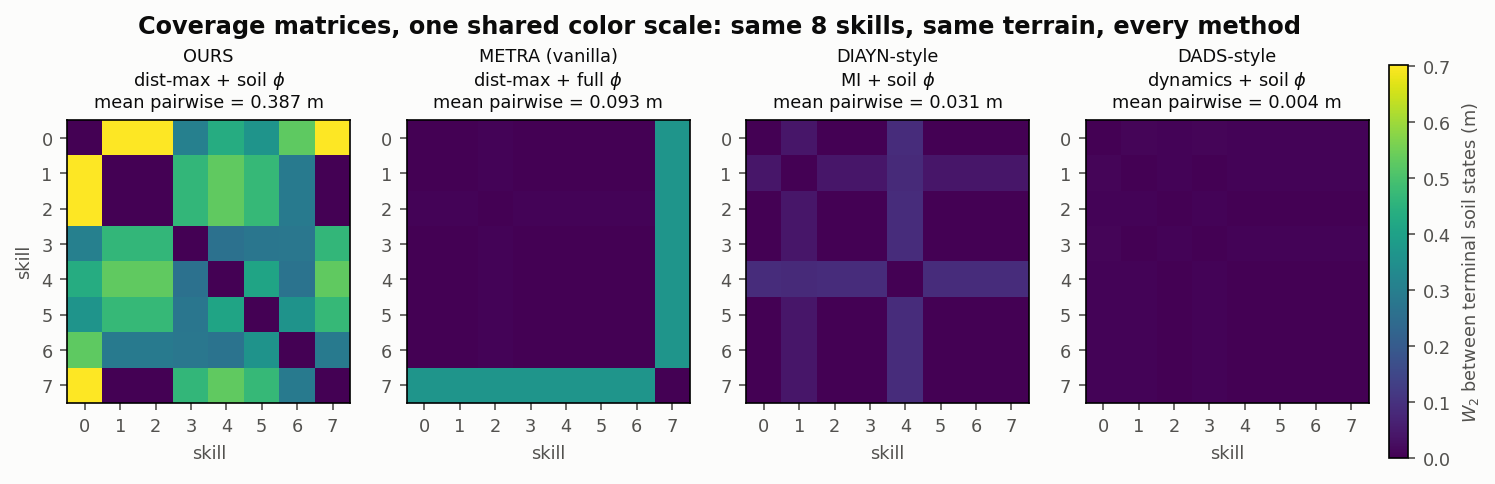
\includegraphics[width=0.98\linewidth]{fig_coverage_matrices.png}
\caption{Pairwise-$W_2$ coverage matrices, same 8 skills, same terrain, shared
color scale. The mean of each matrix's off-diagonal is that method's coverage
score in the frontier table.}
\label{fig:covmats}
\end{figure}

% ============================================================
\section{What is actually new here (novelty statement)}
% ============================================================

\begin{enumerate}[leftmargin=6mm]
\item \textbf{First demonstration of reward-free skill discovery on granular
media.} Digging, piling, and directed transport emerge with no rewards; prior
USD work covers locomotion and rigid objects only.
\item \textbf{The two-ingredient law with a $3\times2\times$seeds factorial.}
Cumulative (distance-maximizing) objectives \emph{and} external-only
conditioning are each necessary, jointly sufficient; $8\times$ effect size.
To our knowledge the first controlled factorial of objective family $\times$
discriminator conditioning anywhere in USD.
\item \textbf{Metric-agnosticism, measured and explained.} Within the working
cell the ground metric is irrelevant (three-way tie), because every $\phi$
becomes a $0.99$-isometry of physical transport regardless --- an emergent-geometry
result that runs \emph{counter} to the METRA lineage's emphasis (and to our own
original hypothesis, which we falsified with pre-registered ablations).
\item \textbf{The slow-state failure taxonomy} --- saturation (MI) / starvation
(dynamics) / telescoping (distance-max) --- turning three unrelated-looking
failures into one design law for material manipulation objectives.
\item \textbf{Certified zero-shot shaping.} Latent steering achieves 39--63\%
goal-distance reduction with $\sim$90\% monotone contraction and a measurable
granularity radius $r(\varepsilon)$ --- the quantitative boundary between what
skill composition can and cannot reach ($=$ ``diversity $\neq$ controllability,''
with a number).
\end{enumerate}

% ============================================================
\section{Limitations and what comes next}
% ============================================================

\textbf{Limitations, plainly.} One domain family in one custom simulator; the
1D measure dominates (vertical structure underexplored --- and the one 2D-metric
run failed by starvation, unexplained at the optimization level); skill
granularity $\approx 0.2$\,m bounds precision; fixed base bounds reachability;
sample sizes are 2--3 seeds per cell (effect sizes are large relative to
seed noise, but more seeds are cheap insurance); the MI cell is DIAYN-style
skill-MI, not MUSIC's agent--surroundings MI (a faithful MUSIC variant remains
to be run).

\medskip
\textbf{Next steps, in order of importance.}
\begin{enumerate}[leftmargin=6mm]
\item \emph{Second material} (2D dough/plasticine): the objective ports
unchanged; success turns the two-ingredient law from a finding about soil into
a principle about materials.
\item \emph{Mobile base $+$ goal-conditioned layer warm-started from skills}:
removes the two mechanical/precision limits; the from-scratch control
experiment already shows the warm start is the necessary half.
\item \emph{Contraction theorem}: formalize ``$\varepsilon$-coverage of
transport directions $\Rightarrow$ geometric $W_2$ contraction to radius
$r(\varepsilon)$'' --- the 90\%-monotone data is its empirical half.
\item \emph{Write-up}: empirical paper (CoRL/RSS shape) around items 1--3.
\end{enumerate}

% ============================================================
\appendix
\section{Appendix: reproduction guide}
% ============================================================

\textbf{Hyperparameters (all runs).} SAC: lr $3{\cdot}10^{-4}$, batch 256,
$\gamma\,0.99$, $\tau\,0.005$, auto-tuned $\alpha$ (target entropy $-3$), twin
critics, buffer $3{\cdot}10^5$. Networks: 2-hidden-layer MLPs, width 256
($\sim$315k parameters total per model). TMSD: skill dim 4 (pilot: 2), dual lr
$10^{-3}$, $\lambda_0 = 30$, relative slack $0.25$, reward scale 100 ($W_2$
rewards are $\sim$$10^{-3}$\,m per step and would drown in SAC's entropy term
otherwise), $W_2$ quadrature 2048 quantiles. DADS: $\sigma = 0.01$, $L = 16$.
Episodes 200 steps; terrain randomization: random cosine height envelope scaled
to bed height.

\medskip
\textbf{Key commands.}
\begin{itemize}[leftmargin=6mm]\small
\item Train: \texttt{python scripts/train\_tmsd.py --steps 200000 --skill-dim 4
--randomize-terrain [--metric w2|euclidean|temporal|sliced\_w2]
[--objective metra|mi|dads] [--phi-input hist|obs] [--measure 1d|2d]}
\item Evaluate (frozen protocol): \texttt{python scripts/compare\_runs.py --all-batch}
\item Goal-reaching study: \texttt{python scripts/eval\_goal\_reaching.py}
\item Demos: \texttt{python scripts/showcase.py} (3-act public demo),
\texttt{python scripts/demo\_excavate\_dump.py --dig 7 9 --dump 4.5 6.5 --live},
\texttt{python scripts/interactive\_demo.py}
\item All figures in this report: \texttt{python report/make\_figures.py}
\end{itemize}

\medskip
\textbf{Data inventory.} 33 runs under \texttt{runs/}: per-run \texttt{log.csv}
(training telemetry), \texttt{episodes.csv} (per-episode soil transport),
checkpoints; \texttt{runs/compare\_summary.csv} (frozen-protocol scores, both
yardsticks); \texttt{runs/full\_comparison.csv} (configs, parameter counts,
wall-clock, throughput, eval merge); \texttt{runs/goal\_eval/} (steering and
isometry data). Narrative documents: \texttt{Ideation.md} (the original plan and
its pre-registered pivot rules), \texttt{Findings.md} (the verdict trail),
\texttt{Comparison.md} (the final table).

\end{document}
